\documentclass{ltjsarticle}
% helper.tex

% You need to rewrite this file to fit your build environment.

% Notice
% The driver of graphicx package is luatex.
% If you use another engine, then you need to rewrite it to your driver.
% For example, if you use pdflatex, then the driver is pdftex.

% Packages
\usepackage{amsmath,amssymb}
\usepackage[luatex]{graphicx}
\usepackage{tikz}
\usetikzlibrary{calc}
\usetikzlibrary{topaths}
\usetikzlibrary{plotmarks}
\usetikzlibrary{intersections}
\usetikzlibrary{arrows,decorations.pathmorphing,backgrounds,positioning,fit,petri}
\usetikzlibrary{arrows.meta}
\usetikzlibrary{3d}

\usepackage{fancybox}
\usepackage{booktabs}

\usepackage[margin=2.4cm]{geometry}

\usepackage[colorlinks=true,linkcolor=black]{hyperref}

% Sample macro.
%\newcommand{\solution}{\begin{flushleft}\textbf{Solution:}\end{flushleft}}
%\newcommand{\proof}{\begin{flushleft}\textbf{Proof}\end{flushleft}}
%\newcommand{\qed}{\begin{flushright}\textbf{q. e. d.}\end{flushright}}
%\newcommand{\answer}[1]{\begin{flushleft}\textbf{Exercise~\ref{#1}}\end{flushleft}}

% Theorem environment.
%\newtheorem{theorem}{Theorem}[section]
%\newtheorem{lemma}{Lemma}[section]
%\newtheorem{corollary}{Corollary}[section]
%\newtheorem{definition}{Definition}[section]
%\newtheorem{example}{Example}[section]
%\newtheorem{exercise}{Exercise}[section]

\title{チュートリアル}
\author{関谷 敏雄} % Write your name if necessary.
\begin{document}
\maketitle
% If you want table of contents here, uncomment the following line.
\tableofcontents

\begin{abstract}
このチュートリアルには9つのセクションがある。
チュートリアルとしての内容はセクション1からセクション8までに書かれている。
最後のセクション9はBuildtoolsのソースファイルに含まれるReadme.ja.mdのコピーである。
\end{abstract}

\section{インストール}
  \subsection{Prerequisite}
Buildtools requires the following items.
\begin{enumerate}
\item Linux OS and bash
\item LaTeX system
\item Make or Rake
\end{enumerate}

\subsubsection{Linux OS and bash}
Buildtools is tested on Debian and Ubuntu.
However, it probably works on other linux distributions.
Bash is required because the shell scripts in Buildtools include bash commands.
\subsubsection{LaTeX system}
There are two options to install LaTeX.

One is installing the LaTeX applications provided by your distribution.
If your distribution is Ubuntu, you can install it by typing the following line.
\begin{verbatim}
$ sudo apt-get install texlive-full
\end{verbatim}
If you have another distribution, refer to the distribution's document to install.

The other way is installing TexLive from \url{https://www.tug.org/texlive}
Refer the documentations in the web to install TexLive system.

\subsubsection{Make or rake}
These applications are not necessarily required to run the tools in Buildtools.
However, it is recommended that they should be used under the control of make or rake.
You don't need to install both of them.
Choose one which you like.

Make is a traditional build tool originally aimed at C compiler.
In Ubuntu, type the following line to install make.
\begin{verbatim}
$ sudo apt-get install make
\end{verbatim}

Rake is a build tool similar to make.
It is one of the ruby application.
The advantage to use rake is that you can put any ruby codes into Rakefile, which is the script file of rake.
Generally speaking, Rakefile is easy to understand than Makefile.
In Ubuntu, type the following line to install rake.
\begin{verbatim}
$ sudo apt-get install rake
\end{verbatim}

If you want to install the latest version of ruby, use rbenv and ruby-build.
See the following github repository and refer to the documentations there.
\begin{itemize}
\item \url{https://github.com/rbenv/rbenv}
\item \url{https://github.com/rbenv/ruby-build}
\end{itemize}

\subsection{Installation}
\subsubsection{Download}
First, access the following github repository.
\begin{itemize}
\item \url{https://github.com/ToshioCP/LaTeX-BuildTools}
\end{itemize}
Click the \verb|Code| button, then popup menu appears.
Click \verb|DOWNLOAD ZIP| menu.
Unzip the download zip file.
\subsubsection{Installation}
Open your terminal.
Change your current directory into the directory you extracted the zip file. 
Then type:
\begin{verbatim}
$ bash install.sh
\end{verbatim}
This script installs the executable files into \verb|\$HOME/bin|.
Debian and Ubuntu adds the directory \verb|\$HOME/bin| into \verb|PATH| environment variable if it exists at the login time.
The script makes the directory \verb|\$HOME/bin| if it doesn't exist.
In that case, you need to re-login to put the directory into the \verb|PATH| environment variable.
This installs scripts into your private directory, so any other users can't access the scripts.
This is called user level installation or private installation.

If you want to install the scripts in \verb|/user/local/bin|, you need to have root privilege.
If your OS is ubuntu, then type:
\begin{verbatim}
$ sudo bash install.sh
\end{verbatim}


\section{lbを使ったコンパイル}
  \subsection{First step}
Lb is the main script in Buildtools.
This section describes how to use it with a small example.

First, make a directory named \verb|example| and change your current directory to it.
\begin{verbatim}
$ makedir example
$ cd example
\end{verbatim}

Then make a tex source file in the directory.
Run your favourite editor and copy the following text, then save it as the name \verb|main.tex|.
\begin{verbatim}
\documentclass{article}
\begin{document}
Hello \LaTeX !!
\end{document}
\end{verbatim}

Then, just type \verb|lb|.
\begin{verbatim}
$ lb
\end{verbatim}
Then, it runs latexmk and pdflatex and compile \verb|main.tex| with them.
Messages appear on your screen, and that shows the process of the compilation.
If there is a line 
\begin{verbatim}
Output written on _build/main.pdf (1 page, 19263 bytes).
\end{verbatim}
then the compilation completes correctly.
Check the directory.
\begin{verbatim}
$ ls -l
total 8
drwxrwxr-x 2 user user 4096 Dec  6 11:59 _build
-rw-rw-r-- 1 user user   72 Dec  6 11:59 main.tex
\end{verbatim}
A new directory \verb|_build| is generated.
Look at the files in the directory.
\begin{verbatim}
$ cd _build
$ ls
\end{verbatim}
There are auxliary files and the target file \verb|main.pdf|.
See \verb|main.pdf| with your pdf-viewer, for example evince.
\begin{verbatim}
$ evince main.pdf
\end{verbatim}
\begin{center}
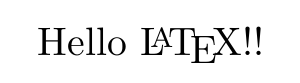
\includegraphics[width=3cm]{hellolatex.png}
\end{center}

\subsection{Use lb.conf}
In the previous subsection, lb runs pdflatex.
The reason why lb chose pdflatex is the documentclass `article'.
It can also be compiled by lualatex or xelatex, but pdflatex has been a standard latex engine for ages.

If you want to use, for example, lualatex to compile, you need to specify it in \verb|lb.conf|.
This configuration file has six items.
\begin{description}
\item[rootfile] Rootfile is the main tex file, which usually includes {\textbackslash}begin\{document\} and {\textbackslash}end\{document\}. Other tex files are called `subfile'.
\item[builddir] This is a temporary directory includes all the auxliary files and the target file, which is usually a pdf file.
\item[engine] This specifies a latex engine, which is one of pdflatex, xelatex, lualatex, latex and platex.
\item[latex\_option] This specifies options to give \verb|latexmk|. The option `-halt-on-error' is given to \verb|latexmk| even if lb.conf doesn't exist.
\item[dvipdf] This is a program which converts dvi into pdf, which is used only with latex or platex. It is unnecessary with other latex engines. `dvipdfmx' is the best at present.
\item[preview] Pdf viewer. This is used to preview the pdf file when lb is given a subfile as an argument.
\end{description}

Run your editor, type the following and save it as the name \verb|lb.conf|.
\begin{verbatim}
rootfile=main
builddir=_build
engine=lualatex
latex_option=-halt-on-error
dvipdf=
preview=evince
\end{verbatim}
Then, type
\begin{verbatim}
$ lb
\end{verbatim}
it used lualatex to compile.

If you want to change the name of the tex file to `example.tex', then modify the first line in lb.conf to
\begin{verbatim}
rootfile=example
\end{verbatim}
or
\begin{verbatim}
rootfile=example.tex
\end{verbatim}
The suffix can be left out.

In addition, if you want to put all the axiliary files and the target file in the source directory, change the second line in lb.conf to:
\begin{verbatim}
builddir=
\end{verbatim}
This specifies null string for builddir item and that means no build directory is made.

Let's try to run \verb|lb| with the following \verb|lb.conf|.
\begin{verbatim}
rootfile=example
builddir=
engine=latex
latex_option=-halt-on-error
dvipdf=dvipdfmx
preview=evince
\end{verbatim}
Now, the engine is latex and dvipdf program is dvipdfmx.
\begin{verbatim}
$ rm -r _build
$ mv main.tex example.tex
$ lb
\end{verbatim}
Then messages appear.
It includes the following line.
\begin{verbatim}
This is pdfTeX, Version 3.14159265-2.6-1.40.21 (TeX Live 2020)
 (preloaded format=latex)
  ... ...
  ... ...
Output written on example.dvi (1 page, 332 bytes).
Transcript written on example.log.
Latexmk: Examining 'example.log'
=== TeX engine is 'pdfTeX'
Latexmk: Log file says output to 'example.dvi'
Latexmk: All targets (example.dvi) are up-to-date
example.dvi -> example.pdf
[1]
3662 bytes written
\end{verbatim}
This tells us that the engine was `latex'%
\footnote{
In Texlive2020, `latex' command calls `pdftex' instead of `tex' which is the original TeX program.
}.
It generates dvi file instead of pdf file.
After that, dvipdfmx is run by latexmk and it translates the dvi file into a pdf file.
The name `dvipdfmx' doesn't appear in the message but `example.dvi -{\textgreater} example.pdf' is outputed by dvipdfmx.
So we know that dvipdfmx was run by latexmk in the build process.
\begin{verbatim}
$ ls
example.aux  example.fdb_latexmk  example.log  example.tex
example.dvi  example.fls          example.pdf  lb.conf
\end{verbatim}
There's no temprary directory like \_build because we specified null string for builddir.

One of the important feature of lb is compiling a subfile separately.
This will be explained in the section  \ref{sec:testcompile} `Test compile' (p. \pageref{sec:testcompile}).

\section{テンプレートの生成}
  \subsection{newtex.conf}
newtexスクリプトはディレクトリを作成し、その中にテンプレートファイルを生成する。
これはコンパイルに先がけて最初に実行される。

はじめに、コンフィギュレーション・ファイルのnewtex.confを作成する必要がある。
Buildtoolsの(ダウンロードした)ソースファイルの中に、newtex.ja.confがある。
このチュートリアルの実行用のディレクトリを作って、その中にこのファイルをコピーする。
\begin{verbatim}
$ cp newtex.ja.conf (作成したディレクトリ)/newtex.conf
\end{verbatim}
コピーが完了したら、ファイルの内容を確認しよう。
\begin{verbatim}
# This is a configuration file for newtex.
# The name of this file is newtex.conf
# A string between # and new line is a commnet and it is ignored by newtex.
# Empty line is also ignored. 

title="チュートリアル"
# document name

# lb.conf
# Lb.conf has six lines.
# The following six lines are copied to lb.conf.
rootfile=main.tex
builddir=_build
engine=lualatex
latex_option=-halt-on-error
dvipdf=
preview=evince

# documentclass
documentclass=ltjsarticle

# chapters/sections and subfile names
#   Chapters/sections and subfile names must be surrounded by double quotes.
#   Subfile names have no suffix or ".tex" suffix.
# If your LaTeX file is not big and no subfile is necessary, then leave out
 the following lines.
section="インストール" "installation"
section="lbを使ったコンパイル" "lb"
section="テンプレートの生成" "generate_templates"   # Subfiles are NOT allowed
 to include space characters. Use underscore instead of space. 
section="TeXソースファイルの編集" "edit_tex_files"
section="テスト・コンパイル" "test_compile"
section="プリプロセッシング" "preprocessing"
section="rakeによる自動化" "rake"
section="アーカイブの作成" "tarball"
\end{verbatim}
ここではこのチュートリアルの文書自身をどのように作成するかを説明する。
上記のファイルはこの作成時に用いたnewtex.confと全く同一の内容である。

ハッシュマーク(\#)から改行まではコメントで、newtexはこの部分を無視する。
空行も同様に無視される。
残りの行がnewtexへの指示が書かれたものである。

それぞれの行は「キー=値」の形式になっている。
使われているキーは、以下の通りである。
\begin{description}
\item[title] 作成する文書の表題
\item[rootfile] ルートファイルの名前
\item[builddir] ビルド・ディレクトリの名前
\item[engine] ソースファイルをコンパイルするlatexエンジン
\item[latex\_option] latexエンジンに与えるオプション
\item[dvipdf] dviをpdfに変換するプログラム
\item[preview] pdfビューワ
\item[documentclass] ドキュメントクラスの名前({\textbackslash}documentclassの引数)
\item[chapter] 章とそれに対応するサブファイル
\item[section] セクションとそれに対応するサブファイル
\end{description}
ltjsbookのようなドキュメントクラスを使い、書籍のような大きな文書を作成する場合は、「chapter」と「section」キーを用いる。
ltjsarticleのようなドキュメントクラスを使い、小さな(あるいはさほど大きくない)文書を作る場合は、「section」キーのみを用いる。

\subsection{newtexの実行}
newtex.confの編集が終わり、保存したら、以下のようにタイプする。
\begin{verbatim}
$ newtex
\end{verbatim}
すると、newtexは「チュートリアル」というnewtex.confに記された表題と同じ名前のディレクトリを作る。
おしも、表題に半角の空白文字が含まれている場合は、それらはアンダースコア(\_)に変換される。
例えば、英語の表題で「A tutorial for beginners」は、「A\_tutorial\_for\_beginners」に変換され、それがディレクトリ名となる。
これは、空白文字を含むファイル名が問題を引き起こす場合があるための処理である。
newtexはさらに雛形となるファイルをそのディレクトリの下に生成する。
\begin{verbatim}
$ cd チュートリアル
$ ls
Makefile            generate_templates.tex  preprocessing.tex
Rakefile            helper.tex              rake.tex
_build              installation.tex        tarball.tex
cover.tex           lb.conf                 test_compile.tex
edit_tex_files.tex  lb.tex
gecko.png           main.tex
\end{verbatim}

いくつか重要なファイルを見てみよう。
\begin{verbatim}
$ cat lb.conf
rootfile=main
builddir=_build
engine=lualatex
latex_option=-halt-on-error
dvipdf=
preview=evince
\end{verbatim}
このファイルの内容は、newtex.confの一部のコピーである。
\begin{verbatim}
$ cat main.tex
\documentclass{ltjsarticle}
% helper.tex

% You need to rewrite this file to fit your build environment.

% Notice
% The driver of graphicx package is luatex.
% If you use another engine, then you need to rewrite it to your driver.
% For example, if you use pdflatex, then the driver is pdftex.

% Packages
\usepackage{amsmath,amssymb}
\usepackage[luatex]{graphicx}
\usepackage{tikz}
\usetikzlibrary{calc}
\usetikzlibrary{topaths}
\usetikzlibrary{plotmarks}
\usetikzlibrary{intersections}
\usetikzlibrary{arrows,decorations.pathmorphing,backgrounds,positioning,fit,petri}
\usetikzlibrary{arrows.meta}
\usetikzlibrary{3d}

\usepackage{fancybox}
\usepackage{booktabs}

\usepackage[margin=2.4cm]{geometry}

\usepackage[colorlinks=true,linkcolor=black]{hyperref}

% Sample macro.
%\newcommand{\solution}{\begin{flushleft}\textbf{Solution:}\end{flushleft}}
%\newcommand{\proof}{\begin{flushleft}\textbf{Proof}\end{flushleft}}
%\newcommand{\qed}{\begin{flushright}\textbf{q. e. d.}\end{flushright}}
%\newcommand{\answer}[1]{\begin{flushleft}\textbf{Exercise~\ref{#1}}\end{flushleft}}

% Theorem environment.
%\newtheorem{theorem}{Theorem}[section]
%\newtheorem{lemma}{Lemma}[section]
%\newtheorem{corollary}{Corollary}[section]
%\newtheorem{definition}{Definition}[section]
%\newtheorem{example}{Example}[section]
%\newtheorem{exercise}{Exercise}[section]

\title{チュートリアル}
\author{} % Write your name if necessary.
\begin{document}
\maketitle
% If you want table of contents here, uncomment the following line.
%\tableofcontents

\section{インストール}
  \subsection{Prerequisite}
Buildtools requires the following items.
\begin{enumerate}
\item Linux OS and bash
\item LaTeX system
\item Make or Rake
\end{enumerate}

\subsubsection{Linux OS and bash}
Buildtools is tested on Debian and Ubuntu.
However, it probably works on other linux distributions.
Bash is required because the shell scripts in Buildtools include bash commands.
\subsubsection{LaTeX system}
There are two options to install LaTeX.

One is installing the LaTeX applications provided by your distribution.
If your distribution is Ubuntu, you can install it by typing the following line.
\begin{verbatim}
$ sudo apt-get install texlive-full
\end{verbatim}
If you have another distribution, refer to the distribution's document to install.

The other way is installing TexLive from \url{https://www.tug.org/texlive}
Refer the documentations in the web to install TexLive system.

\subsubsection{Make or rake}
These applications are not necessarily required to run the tools in Buildtools.
However, it is recommended that they should be used under the control of make or rake.
You don't need to install both of them.
Choose one which you like.

Make is a traditional build tool originally aimed at C compiler.
In Ubuntu, type the following line to install make.
\begin{verbatim}
$ sudo apt-get install make
\end{verbatim}

Rake is a build tool similar to make.
It is one of the ruby application.
The advantage to use rake is that you can put any ruby codes into Rakefile, which is the script file of rake.
Generally speaking, Rakefile is easy to understand than Makefile.
In Ubuntu, type the following line to install rake.
\begin{verbatim}
$ sudo apt-get install rake
\end{verbatim}

If you want to install the latest version of ruby, use rbenv and ruby-build.
See the following github repository and refer to the documentations there.
\begin{itemize}
\item \url{https://github.com/rbenv/rbenv}
\item \url{https://github.com/rbenv/ruby-build}
\end{itemize}

\subsection{Installation}
\subsubsection{Download}
First, access the following github repository.
\begin{itemize}
\item \url{https://github.com/ToshioCP/LaTeX-BuildTools}
\end{itemize}
Click the \verb|Code| button, then popup menu appears.
Click \verb|DOWNLOAD ZIP| menu.
Unzip the download zip file.
\subsubsection{Installation}
Open your terminal.
Change your current directory into the directory you extracted the zip file. 
Then type:
\begin{verbatim}
$ bash install.sh
\end{verbatim}
This script installs the executable files into \verb|\$HOME/bin|.
Debian and Ubuntu adds the directory \verb|\$HOME/bin| into \verb|PATH| environment variable if it exists at the login time.
The script makes the directory \verb|\$HOME/bin| if it doesn't exist.
In that case, you need to re-login to put the directory into the \verb|PATH| environment variable.
This installs scripts into your private directory, so any other users can't access the scripts.
This is called user level installation or private installation.

If you want to install the scripts in \verb|/user/local/bin|, you need to have root privilege.
If your OS is ubuntu, then type:
\begin{verbatim}
$ sudo bash install.sh
\end{verbatim}


\section{lbを使ったコンパイル}
  \subsection{First step}
Lb is the main script in Buildtools.
This section describes how to use it with a small example.

First, make a directory named \verb|example| and change your current directory to it.
\begin{verbatim}
$ makedir example
$ cd example
\end{verbatim}

Then make a tex source file in the directory.
Run your favourite editor and copy the following text, then save it as the name \verb|main.tex|.
\begin{verbatim}
\documentclass{article}
\begin{document}
Hello \LaTeX !!
\end{document}
\end{verbatim}

Then, just type \verb|lb|.
\begin{verbatim}
$ lb
\end{verbatim}
Then, it runs latexmk and pdflatex and compile \verb|main.tex| with them.
Messages appear on your screen, and that shows the process of the compilation.
If there is a line 
\begin{verbatim}
Output written on _build/main.pdf (1 page, 19263 bytes).
\end{verbatim}
then the compilation completes correctly.
Check the directory.
\begin{verbatim}
$ ls -l
total 8
drwxrwxr-x 2 user user 4096 Dec  6 11:59 _build
-rw-rw-r-- 1 user user   72 Dec  6 11:59 main.tex
\end{verbatim}
A new directory \verb|_build| is generated.
Look at the files in the directory.
\begin{verbatim}
$ cd _build
$ ls
\end{verbatim}
There are auxliary files and the target file \verb|main.pdf|.
See \verb|main.pdf| with your pdf-viewer, for example evince.
\begin{verbatim}
$ evince main.pdf
\end{verbatim}
\begin{center}
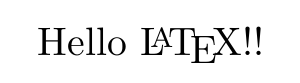
\includegraphics[width=3cm]{hellolatex.png}
\end{center}

\subsection{Use lb.conf}
In the previous subsection, lb runs pdflatex.
The reason why lb chose pdflatex is the documentclass `article'.
It can also be compiled by lualatex or xelatex, but pdflatex has been a standard latex engine for ages.

If you want to use, for example, lualatex to compile, you need to specify it in \verb|lb.conf|.
This configuration file has six items.
\begin{description}
\item[rootfile] Rootfile is the main tex file, which usually includes {\textbackslash}begin\{document\} and {\textbackslash}end\{document\}. Other tex files are called `subfile'.
\item[builddir] This is a temporary directory includes all the auxliary files and the target file, which is usually a pdf file.
\item[engine] This specifies a latex engine, which is one of pdflatex, xelatex, lualatex, latex and platex.
\item[latex\_option] This specifies options to give \verb|latexmk|. The option `-halt-on-error' is given to \verb|latexmk| even if lb.conf doesn't exist.
\item[dvipdf] This is a program which converts dvi into pdf, which is used only with latex or platex. It is unnecessary with other latex engines. `dvipdfmx' is the best at present.
\item[preview] Pdf viewer. This is used to preview the pdf file when lb is given a subfile as an argument.
\end{description}

Run your editor, type the following and save it as the name \verb|lb.conf|.
\begin{verbatim}
rootfile=main
builddir=_build
engine=lualatex
latex_option=-halt-on-error
dvipdf=
preview=evince
\end{verbatim}
Then, type
\begin{verbatim}
$ lb
\end{verbatim}
it used lualatex to compile.

If you want to change the name of the tex file to `example.tex', then modify the first line in lb.conf to
\begin{verbatim}
rootfile=example
\end{verbatim}
or
\begin{verbatim}
rootfile=example.tex
\end{verbatim}
The suffix can be left out.

In addition, if you want to put all the axiliary files and the target file in the source directory, change the second line in lb.conf to:
\begin{verbatim}
builddir=
\end{verbatim}
This specifies null string for builddir item and that means no build directory is made.

Let's try to run \verb|lb| with the following \verb|lb.conf|.
\begin{verbatim}
rootfile=example
builddir=
engine=latex
latex_option=-halt-on-error
dvipdf=dvipdfmx
preview=evince
\end{verbatim}
Now, the engine is latex and dvipdf program is dvipdfmx.
\begin{verbatim}
$ rm -r _build
$ mv main.tex example.tex
$ lb
\end{verbatim}
Then messages appear.
It includes the following line.
\begin{verbatim}
This is pdfTeX, Version 3.14159265-2.6-1.40.21 (TeX Live 2020)
 (preloaded format=latex)
  ... ...
  ... ...
Output written on example.dvi (1 page, 332 bytes).
Transcript written on example.log.
Latexmk: Examining 'example.log'
=== TeX engine is 'pdfTeX'
Latexmk: Log file says output to 'example.dvi'
Latexmk: All targets (example.dvi) are up-to-date
example.dvi -> example.pdf
[1]
3662 bytes written
\end{verbatim}
This tells us that the engine was `latex'%
\footnote{
In Texlive2020, `latex' command calls `pdftex' instead of `tex' which is the original TeX program.
}.
It generates dvi file instead of pdf file.
After that, dvipdfmx is run by latexmk and it translates the dvi file into a pdf file.
The name `dvipdfmx' doesn't appear in the message but `example.dvi -{\textgreater} example.pdf' is outputed by dvipdfmx.
So we know that dvipdfmx was run by latexmk in the build process.
\begin{verbatim}
$ ls
example.aux  example.fdb_latexmk  example.log  example.tex
example.dvi  example.fls          example.pdf  lb.conf
\end{verbatim}
There's no temprary directory like \_build because we specified null string for builddir.

One of the important feature of lb is compiling a subfile separately.
This will be explained in the section  \ref{sec:testcompile} `Test compile' (p. \pageref{sec:testcompile}).

\section{テンプレートの生成}
  \subsection{newtex.conf}
newtexスクリプトはディレクトリを作成し、その中にテンプレートファイルを生成する。
これはコンパイルに先がけて最初に実行される。

はじめに、コンフィギュレーション・ファイルのnewtex.confを作成する必要がある。
Buildtoolsの(ダウンロードした)ソースファイルの中に、newtex.ja.confがある。
このチュートリアルの実行用のディレクトリを作って、その中にこのファイルをコピーする。
\begin{verbatim}
$ cp newtex.ja.conf (作成したディレクトリ)/newtex.conf
\end{verbatim}
コピーが完了したら、ファイルの内容を確認しよう。
\begin{verbatim}
# This is a configuration file for newtex.
# The name of this file is newtex.conf
# A string between # and new line is a commnet and it is ignored by newtex.
# Empty line is also ignored. 

title="チュートリアル"
# document name

# lb.conf
# Lb.conf has six lines.
# The following six lines are copied to lb.conf.
rootfile=main.tex
builddir=_build
engine=lualatex
latex_option=-halt-on-error
dvipdf=
preview=evince

# documentclass
documentclass=ltjsarticle

# chapters/sections and subfile names
#   Chapters/sections and subfile names must be surrounded by double quotes.
#   Subfile names have no suffix or ".tex" suffix.
# If your LaTeX file is not big and no subfile is necessary, then leave out
 the following lines.
section="インストール" "installation"
section="lbを使ったコンパイル" "lb"
section="テンプレートの生成" "generate_templates"   # Subfiles are NOT allowed
 to include space characters. Use underscore instead of space. 
section="TeXソースファイルの編集" "edit_tex_files"
section="テスト・コンパイル" "test_compile"
section="プリプロセッシング" "preprocessing"
section="rakeによる自動化" "rake"
section="アーカイブの作成" "tarball"
\end{verbatim}
ここではこのチュートリアルの文書自身をどのように作成するかを説明する。
上記のファイルはこの作成時に用いたnewtex.confと全く同一の内容である。

ハッシュマーク(\#)から改行まではコメントで、newtexはこの部分を無視する。
空行も同様に無視される。
残りの行がnewtexへの指示が書かれたものである。

それぞれの行は「キー=値」の形式になっている。
使われているキーは、以下の通りである。
\begin{description}
\item[title] 作成する文書の表題
\item[rootfile] ルートファイルの名前
\item[builddir] ビルド・ディレクトリの名前
\item[engine] ソースファイルをコンパイルするlatexエンジン
\item[latex\_option] latexエンジンに与えるオプション
\item[dvipdf] dviをpdfに変換するプログラム
\item[preview] pdfビューワ
\item[documentclass] ドキュメントクラスの名前({\textbackslash}documentclassの引数)
\item[chapter] 章とそれに対応するサブファイル
\item[section] セクションとそれに対応するサブファイル
\end{description}
ltjsbookのようなドキュメントクラスを使い、書籍のような大きな文書を作成する場合は、「chapter」と「section」キーを用いる。
ltjsarticleのようなドキュメントクラスを使い、小さな(あるいはさほど大きくない)文書を作る場合は、「section」キーのみを用いる。

\subsection{newtexの実行}
newtex.confの編集が終わり、保存したら、以下のようにタイプする。
\begin{verbatim}
$ newtex
\end{verbatim}
すると、newtexは「チュートリアル」というnewtex.confに記された表題と同じ名前のディレクトリを作る。
おしも、表題に半角の空白文字が含まれている場合は、それらはアンダースコア(\_)に変換される。
例えば、英語の表題で「A tutorial for beginners」は、「A\_tutorial\_for\_beginners」に変換され、それがディレクトリ名となる。
これは、空白文字を含むファイル名が問題を引き起こす場合があるための処理である。
newtexはさらに雛形となるファイルをそのディレクトリの下に生成する。
\begin{verbatim}
$ cd チュートリアル
$ ls
Makefile            generate_templates.tex  preprocessing.tex
Rakefile            helper.tex              rake.tex
_build              installation.tex        tarball.tex
cover.tex           lb.conf                 test_compile.tex
edit_tex_files.tex  lb.tex
gecko.png           main.tex
\end{verbatim}

いくつか重要なファイルを見てみよう。
\begin{verbatim}
$ cat lb.conf
rootfile=main
builddir=_build
engine=lualatex
latex_option=-halt-on-error
dvipdf=
preview=evince
\end{verbatim}
このファイルの内容は、newtex.confの一部のコピーである。
\begin{verbatim}
$ cat main.tex
\documentclass{ltjsarticle}
% helper.tex

% You need to rewrite this file to fit your build environment.

% Notice
% The driver of graphicx package is luatex.
% If you use another engine, then you need to rewrite it to your driver.
% For example, if you use pdflatex, then the driver is pdftex.

% Packages
\usepackage{amsmath,amssymb}
\usepackage[luatex]{graphicx}
\usepackage{tikz}
\usetikzlibrary{calc}
\usetikzlibrary{topaths}
\usetikzlibrary{plotmarks}
\usetikzlibrary{intersections}
\usetikzlibrary{arrows,decorations.pathmorphing,backgrounds,positioning,fit,petri}
\usetikzlibrary{arrows.meta}
\usetikzlibrary{3d}

\usepackage{fancybox}
\usepackage{booktabs}

\usepackage[margin=2.4cm]{geometry}

\usepackage[colorlinks=true,linkcolor=black]{hyperref}

% Sample macro.
%\newcommand{\solution}{\begin{flushleft}\textbf{Solution:}\end{flushleft}}
%\newcommand{\proof}{\begin{flushleft}\textbf{Proof}\end{flushleft}}
%\newcommand{\qed}{\begin{flushright}\textbf{q. e. d.}\end{flushright}}
%\newcommand{\answer}[1]{\begin{flushleft}\textbf{Exercise~\ref{#1}}\end{flushleft}}

% Theorem environment.
%\newtheorem{theorem}{Theorem}[section]
%\newtheorem{lemma}{Lemma}[section]
%\newtheorem{corollary}{Corollary}[section]
%\newtheorem{definition}{Definition}[section]
%\newtheorem{example}{Example}[section]
%\newtheorem{exercise}{Exercise}[section]

\title{チュートリアル}
\author{} % Write your name if necessary.
\begin{document}
\maketitle
% If you want table of contents here, uncomment the following line.
%\tableofcontents

\section{インストール}
  \subsection{Prerequisite}
Buildtools requires the following items.
\begin{enumerate}
\item Linux OS and bash
\item LaTeX system
\item Make or Rake
\end{enumerate}

\subsubsection{Linux OS and bash}
Buildtools is tested on Debian and Ubuntu.
However, it probably works on other linux distributions.
Bash is required because the shell scripts in Buildtools include bash commands.
\subsubsection{LaTeX system}
There are two options to install LaTeX.

One is installing the LaTeX applications provided by your distribution.
If your distribution is Ubuntu, you can install it by typing the following line.
\begin{verbatim}
$ sudo apt-get install texlive-full
\end{verbatim}
If you have another distribution, refer to the distribution's document to install.

The other way is installing TexLive from \url{https://www.tug.org/texlive}
Refer the documentations in the web to install TexLive system.

\subsubsection{Make or rake}
These applications are not necessarily required to run the tools in Buildtools.
However, it is recommended that they should be used under the control of make or rake.
You don't need to install both of them.
Choose one which you like.

Make is a traditional build tool originally aimed at C compiler.
In Ubuntu, type the following line to install make.
\begin{verbatim}
$ sudo apt-get install make
\end{verbatim}

Rake is a build tool similar to make.
It is one of the ruby application.
The advantage to use rake is that you can put any ruby codes into Rakefile, which is the script file of rake.
Generally speaking, Rakefile is easy to understand than Makefile.
In Ubuntu, type the following line to install rake.
\begin{verbatim}
$ sudo apt-get install rake
\end{verbatim}

If you want to install the latest version of ruby, use rbenv and ruby-build.
See the following github repository and refer to the documentations there.
\begin{itemize}
\item \url{https://github.com/rbenv/rbenv}
\item \url{https://github.com/rbenv/ruby-build}
\end{itemize}

\subsection{Installation}
\subsubsection{Download}
First, access the following github repository.
\begin{itemize}
\item \url{https://github.com/ToshioCP/LaTeX-BuildTools}
\end{itemize}
Click the \verb|Code| button, then popup menu appears.
Click \verb|DOWNLOAD ZIP| menu.
Unzip the download zip file.
\subsubsection{Installation}
Open your terminal.
Change your current directory into the directory you extracted the zip file. 
Then type:
\begin{verbatim}
$ bash install.sh
\end{verbatim}
This script installs the executable files into \verb|\$HOME/bin|.
Debian and Ubuntu adds the directory \verb|\$HOME/bin| into \verb|PATH| environment variable if it exists at the login time.
The script makes the directory \verb|\$HOME/bin| if it doesn't exist.
In that case, you need to re-login to put the directory into the \verb|PATH| environment variable.
This installs scripts into your private directory, so any other users can't access the scripts.
This is called user level installation or private installation.

If you want to install the scripts in \verb|/user/local/bin|, you need to have root privilege.
If your OS is ubuntu, then type:
\begin{verbatim}
$ sudo bash install.sh
\end{verbatim}


\section{lbを使ったコンパイル}
  \subsection{First step}
Lb is the main script in Buildtools.
This section describes how to use it with a small example.

First, make a directory named \verb|example| and change your current directory to it.
\begin{verbatim}
$ makedir example
$ cd example
\end{verbatim}

Then make a tex source file in the directory.
Run your favourite editor and copy the following text, then save it as the name \verb|main.tex|.
\begin{verbatim}
\documentclass{article}
\begin{document}
Hello \LaTeX !!
\end{document}
\end{verbatim}

Then, just type \verb|lb|.
\begin{verbatim}
$ lb
\end{verbatim}
Then, it runs latexmk and pdflatex and compile \verb|main.tex| with them.
Messages appear on your screen, and that shows the process of the compilation.
If there is a line 
\begin{verbatim}
Output written on _build/main.pdf (1 page, 19263 bytes).
\end{verbatim}
then the compilation completes correctly.
Check the directory.
\begin{verbatim}
$ ls -l
total 8
drwxrwxr-x 2 user user 4096 Dec  6 11:59 _build
-rw-rw-r-- 1 user user   72 Dec  6 11:59 main.tex
\end{verbatim}
A new directory \verb|_build| is generated.
Look at the files in the directory.
\begin{verbatim}
$ cd _build
$ ls
\end{verbatim}
There are auxliary files and the target file \verb|main.pdf|.
See \verb|main.pdf| with your pdf-viewer, for example evince.
\begin{verbatim}
$ evince main.pdf
\end{verbatim}
\begin{center}
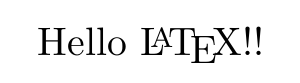
\includegraphics[width=3cm]{hellolatex.png}
\end{center}

\subsection{Use lb.conf}
In the previous subsection, lb runs pdflatex.
The reason why lb chose pdflatex is the documentclass `article'.
It can also be compiled by lualatex or xelatex, but pdflatex has been a standard latex engine for ages.

If you want to use, for example, lualatex to compile, you need to specify it in \verb|lb.conf|.
This configuration file has six items.
\begin{description}
\item[rootfile] Rootfile is the main tex file, which usually includes {\textbackslash}begin\{document\} and {\textbackslash}end\{document\}. Other tex files are called `subfile'.
\item[builddir] This is a temporary directory includes all the auxliary files and the target file, which is usually a pdf file.
\item[engine] This specifies a latex engine, which is one of pdflatex, xelatex, lualatex, latex and platex.
\item[latex\_option] This specifies options to give \verb|latexmk|. The option `-halt-on-error' is given to \verb|latexmk| even if lb.conf doesn't exist.
\item[dvipdf] This is a program which converts dvi into pdf, which is used only with latex or platex. It is unnecessary with other latex engines. `dvipdfmx' is the best at present.
\item[preview] Pdf viewer. This is used to preview the pdf file when lb is given a subfile as an argument.
\end{description}

Run your editor, type the following and save it as the name \verb|lb.conf|.
\begin{verbatim}
rootfile=main
builddir=_build
engine=lualatex
latex_option=-halt-on-error
dvipdf=
preview=evince
\end{verbatim}
Then, type
\begin{verbatim}
$ lb
\end{verbatim}
it used lualatex to compile.

If you want to change the name of the tex file to `example.tex', then modify the first line in lb.conf to
\begin{verbatim}
rootfile=example
\end{verbatim}
or
\begin{verbatim}
rootfile=example.tex
\end{verbatim}
The suffix can be left out.

In addition, if you want to put all the axiliary files and the target file in the source directory, change the second line in lb.conf to:
\begin{verbatim}
builddir=
\end{verbatim}
This specifies null string for builddir item and that means no build directory is made.

Let's try to run \verb|lb| with the following \verb|lb.conf|.
\begin{verbatim}
rootfile=example
builddir=
engine=latex
latex_option=-halt-on-error
dvipdf=dvipdfmx
preview=evince
\end{verbatim}
Now, the engine is latex and dvipdf program is dvipdfmx.
\begin{verbatim}
$ rm -r _build
$ mv main.tex example.tex
$ lb
\end{verbatim}
Then messages appear.
It includes the following line.
\begin{verbatim}
This is pdfTeX, Version 3.14159265-2.6-1.40.21 (TeX Live 2020)
 (preloaded format=latex)
  ... ...
  ... ...
Output written on example.dvi (1 page, 332 bytes).
Transcript written on example.log.
Latexmk: Examining 'example.log'
=== TeX engine is 'pdfTeX'
Latexmk: Log file says output to 'example.dvi'
Latexmk: All targets (example.dvi) are up-to-date
example.dvi -> example.pdf
[1]
3662 bytes written
\end{verbatim}
This tells us that the engine was `latex'%
\footnote{
In Texlive2020, `latex' command calls `pdftex' instead of `tex' which is the original TeX program.
}.
It generates dvi file instead of pdf file.
After that, dvipdfmx is run by latexmk and it translates the dvi file into a pdf file.
The name `dvipdfmx' doesn't appear in the message but `example.dvi -{\textgreater} example.pdf' is outputed by dvipdfmx.
So we know that dvipdfmx was run by latexmk in the build process.
\begin{verbatim}
$ ls
example.aux  example.fdb_latexmk  example.log  example.tex
example.dvi  example.fls          example.pdf  lb.conf
\end{verbatim}
There's no temprary directory like \_build because we specified null string for builddir.

One of the important feature of lb is compiling a subfile separately.
This will be explained in the section  \ref{sec:testcompile} `Test compile' (p. \pageref{sec:testcompile}).

\section{テンプレートの生成}
  \subsection{newtex.conf}
newtexスクリプトはディレクトリを作成し、その中にテンプレートファイルを生成する。
これはコンパイルに先がけて最初に実行される。

はじめに、コンフィギュレーション・ファイルのnewtex.confを作成する必要がある。
Buildtoolsの(ダウンロードした)ソースファイルの中に、newtex.ja.confがある。
このチュートリアルの実行用のディレクトリを作って、その中にこのファイルをコピーする。
\begin{verbatim}
$ cp newtex.ja.conf (作成したディレクトリ)/newtex.conf
\end{verbatim}
コピーが完了したら、ファイルの内容を確認しよう。
\begin{verbatim}
# This is a configuration file for newtex.
# The name of this file is newtex.conf
# A string between # and new line is a commnet and it is ignored by newtex.
# Empty line is also ignored. 

title="チュートリアル"
# document name

# lb.conf
# Lb.conf has six lines.
# The following six lines are copied to lb.conf.
rootfile=main.tex
builddir=_build
engine=lualatex
latex_option=-halt-on-error
dvipdf=
preview=evince

# documentclass
documentclass=ltjsarticle

# chapters/sections and subfile names
#   Chapters/sections and subfile names must be surrounded by double quotes.
#   Subfile names have no suffix or ".tex" suffix.
# If your LaTeX file is not big and no subfile is necessary, then leave out
 the following lines.
section="インストール" "installation"
section="lbを使ったコンパイル" "lb"
section="テンプレートの生成" "generate_templates"   # Subfiles are NOT allowed
 to include space characters. Use underscore instead of space. 
section="TeXソースファイルの編集" "edit_tex_files"
section="テスト・コンパイル" "test_compile"
section="プリプロセッシング" "preprocessing"
section="rakeによる自動化" "rake"
section="アーカイブの作成" "tarball"
\end{verbatim}
ここではこのチュートリアルの文書自身をどのように作成するかを説明する。
上記のファイルはこの作成時に用いたnewtex.confと全く同一の内容である。

ハッシュマーク(\#)から改行まではコメントで、newtexはこの部分を無視する。
空行も同様に無視される。
残りの行がnewtexへの指示が書かれたものである。

それぞれの行は「キー=値」の形式になっている。
使われているキーは、以下の通りである。
\begin{description}
\item[title] 作成する文書の表題
\item[rootfile] ルートファイルの名前
\item[builddir] ビルド・ディレクトリの名前
\item[engine] ソースファイルをコンパイルするlatexエンジン
\item[latex\_option] latexエンジンに与えるオプション
\item[dvipdf] dviをpdfに変換するプログラム
\item[preview] pdfビューワ
\item[documentclass] ドキュメントクラスの名前({\textbackslash}documentclassの引数)
\item[chapter] 章とそれに対応するサブファイル
\item[section] セクションとそれに対応するサブファイル
\end{description}
ltjsbookのようなドキュメントクラスを使い、書籍のような大きな文書を作成する場合は、「chapter」と「section」キーを用いる。
ltjsarticleのようなドキュメントクラスを使い、小さな(あるいはさほど大きくない)文書を作る場合は、「section」キーのみを用いる。

\subsection{newtexの実行}
newtex.confの編集が終わり、保存したら、以下のようにタイプする。
\begin{verbatim}
$ newtex
\end{verbatim}
すると、newtexは「チュートリアル」というnewtex.confに記された表題と同じ名前のディレクトリを作る。
おしも、表題に半角の空白文字が含まれている場合は、それらはアンダースコア(\_)に変換される。
例えば、英語の表題で「A tutorial for beginners」は、「A\_tutorial\_for\_beginners」に変換され、それがディレクトリ名となる。
これは、空白文字を含むファイル名が問題を引き起こす場合があるための処理である。
newtexはさらに雛形となるファイルをそのディレクトリの下に生成する。
\begin{verbatim}
$ cd チュートリアル
$ ls
Makefile            generate_templates.tex  preprocessing.tex
Rakefile            helper.tex              rake.tex
_build              installation.tex        tarball.tex
cover.tex           lb.conf                 test_compile.tex
edit_tex_files.tex  lb.tex
gecko.png           main.tex
\end{verbatim}

いくつか重要なファイルを見てみよう。
\begin{verbatim}
$ cat lb.conf
rootfile=main
builddir=_build
engine=lualatex
latex_option=-halt-on-error
dvipdf=
preview=evince
\end{verbatim}
このファイルの内容は、newtex.confの一部のコピーである。
\begin{verbatim}
$ cat main.tex
\documentclass{ltjsarticle}
\input{helper.tex}
\title{チュートリアル}
\author{} % Write your name if necessary.
\begin{document}
\maketitle
% If you want table of contents here, uncomment the following line.
%\tableofcontents

\section{インストール}
  \input{installation.tex}
\section{lbを使ったコンパイル}
  \input{lb.tex}
\section{テンプレートの生成}
  \input{generate_templates.tex}
\section{TeXソースファイルの編集}
  \input{edit_tex_files.tex}
\section{テスト・コンパイル}
  \input{test_compile.tex}
\section{プリプロセッシング}
  \input{preprocessing.tex}
\section{rakeによる自動化}
  \input{rake.tex}
\section{アーカイブの作成}
  \input{tarball.tex}
\end{document}
\end{verbatim}
最初の行はドキュメントクラスの指定で、newtex.confのdovumentclassキーの値が引数になっている。
2番めの行ではhelper.texを取り込むinputコマンドが書かれている。
helper.texは\verb|\usepackage|コマンドでパッケージを取り込んだり、\verb|\newcommand|コマンドでマクロを定義するなどの役割がある。
プリアンブルの記述のほとんどはhelper.texに書かれている。
ユーザが自分専用のhelper.texを作っておくのは、良い考えである。
というのは、同じプリアンブルをいろいろな文書に使い回すことが多いからである。
自分専用helper.texを持っているユーザはこのテンプレートを上書きすると良い。

4行目は書き直しが必要である。
例えば、
\begin{verbatim}
\author{関谷 敏雄}
\end{verbatim}
のように。
`{\textbackslash}date'、`{\textbackslash}thanks'、abstract環境などを必要に応じて付け加えて良い。
また、目次が必要であれば、8行目のハッシュマークを外して、アンコメントする。
残りの行は、セクションとそのセクションの内容を記述したサブファイルを取り込むための{\textbackslash}inputコマンドである。

Rakefileはrakeに対する指示を書いたファイルである。
当面はこれを書き換える必要はない。
テンプレートをそのまま使い、rakeを実行してみよう。
\begin{verbatim}
$ rake
 ... ...
 ... ...
$ ls
Makefile            generate_templates.tex  preprocessing.tex
Rakefile            helper.tex              rake.tex
_build              installation.tex        tarball.tex
cover.tex           lb.conf                 test_compile.tex
edit_tex_files.tex  lb.tex                  チュートリアル.pdf
gecko.png           main.tex
$ ls _build
main.aux          main.fls  main.out
main.fdb_latexmk  main.log  main.pdf
$ evince Tutorial.pdf
\end{verbatim}
rakeはlbを起動してmain.texをコンパイルし、その後「\_build/main.pdf」を「チュートリアル.pdf」にコピーする。
Evinceは「チュートリアル.pdf」を次のように表示してくれる。
\begin{center}
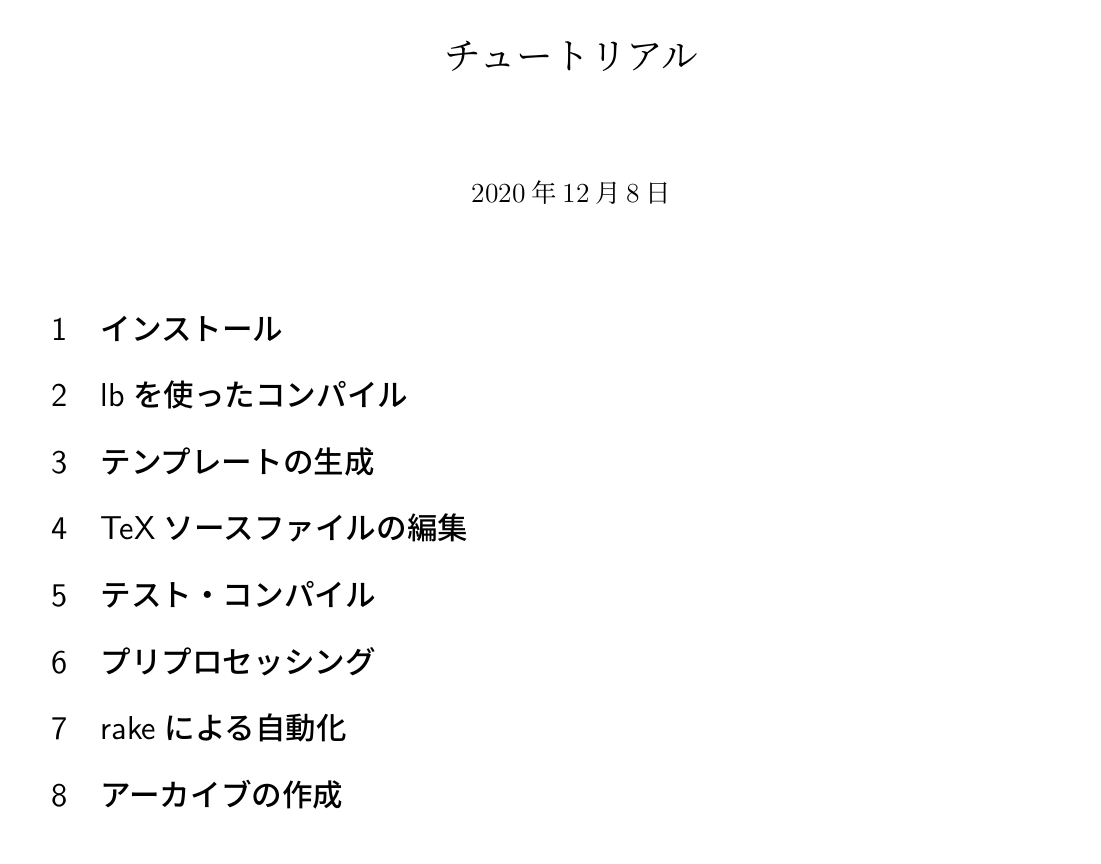
\includegraphics[width=12cm]{Tutorial_1.png}
\end{center}


\section{TeXソースファイルの編集}
  main.texには8つのセクションとそれに対応するサブファイルを取り込む{\textbackslash}inputコマンドが書かれている。
それぞれのサブファイルはテンプレートとして生成された直後は空のファイルである。
そのサブファイルの編集が文書作成の主要な作業になり、作成にかかる時間の大部分がそれに当てられる。

ところで、セクションの編集の途中でも、そこまでをpdfにするとどうなるかを見たいことがあるだろう。
そのためのコンパイルをテスト・コンパイルという。
多くの場合、編集とテスト・コンパイルの間を何回も行ったり来たりしながら、文書作成が進むものである。

もしも、文書がさほど大きくないならば、rakeを用いるのがテスト・コンパイルには最も良い。
というのは、さほどコンパイル時間もかからず、文書全体のpdfを見ることができるからである。
このチュートリアルは、どちらかといえば小さい文書であるから、rakeをテスト・コンパイルに用いるのが良い。

さて、最初のセクションを編集する代わりに、ソースファイル「installation.tex」をコピーしよう。
\begin{verbatim}
\subsection{動作条件}
Buildtoolsには次のものが必要である。
\begin{enumerate}
\item Linux OS とbash
\item LaTeXシステム
\item MakeまたはRake
\end{enumerate}
 ... ...
 ... ...
\end{verbatim}
コピーがすんだら、下記のようにタイプしてpdfを見てみよう。
\begin{verbatim}
$ rake
$ evince チュートリアル.pdf
\end{verbatim}

\begin{center}
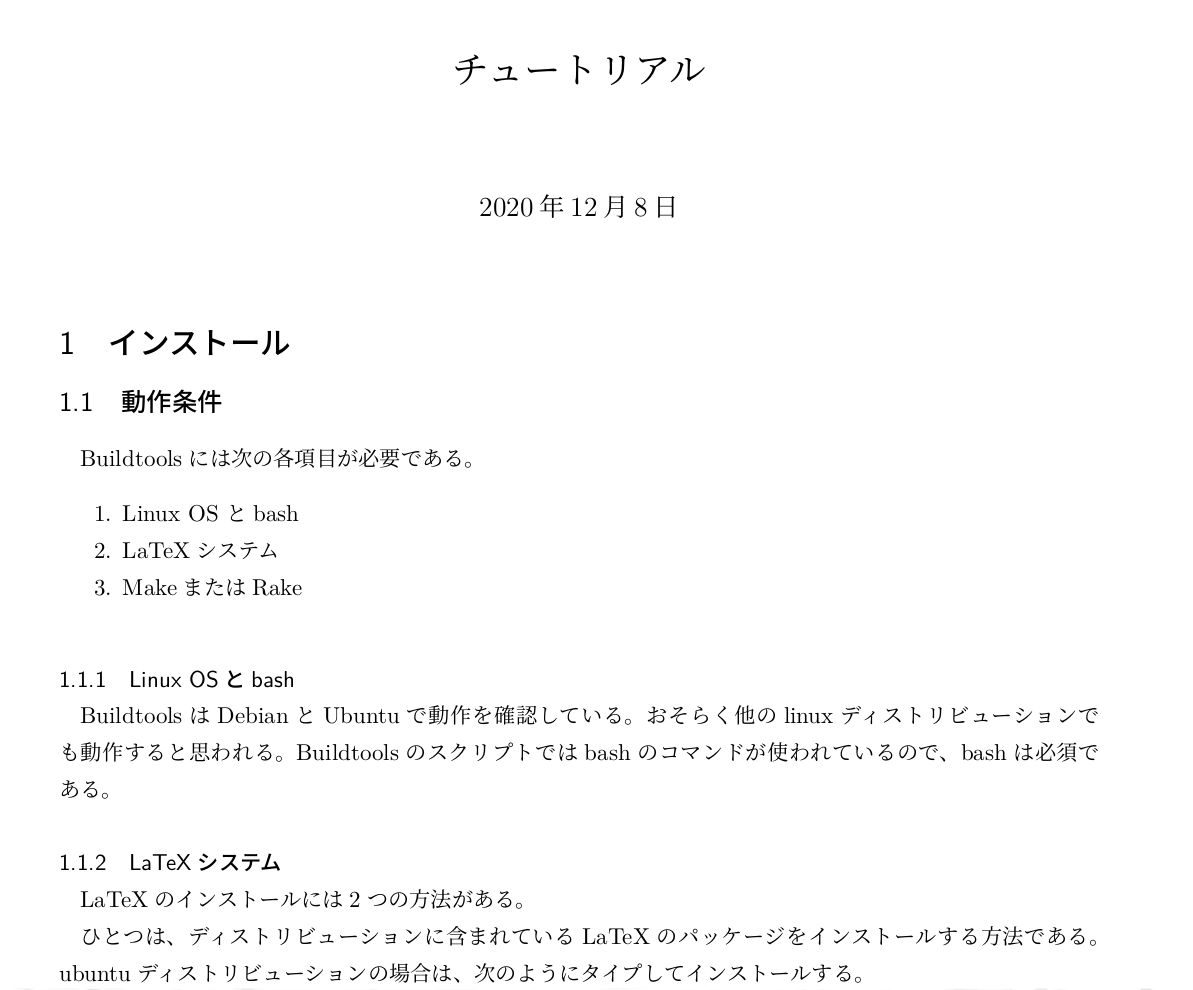
\includegraphics[width=12cm]{Tutorial_2.png}
\end{center}

\section{テスト・コンパイル}
  If you make a big document, for example a book which has more than 100 pages, then using rake is not a good way to test-compile.
The bigger the dicument is, the longer time the compiling takes.

It is a better way to use `lb' to test-compile a subfile separately.
Lb makes a temporary rootfile which includes only the subfile and compile it once.
The advantage of this way is very quick to compile.
However, it has disadvantages.
It only compiles the subfile, so the pdf you get is not a finished document.
It compiles once, so cross-reference doesn't work at all.
It is difficult to say which is better.
it depends on the size of your document.
If it is very big, use lb to test-compile separately.

In this section, I want to show you how to use lb to test-compile a subfile.
This document `Tutorial' is not big, but it's OK.
This is an example to show how to use lb.

Type the following.
\begin{verbatim}
$ lb installation
\end{verbatim}
The argument is a subfile.
The suffix can be left out.
Then, lb makes a temporary rootfile `\_build/test\_installation.tex'.
Its preamble is a copy of the preamble in the original rootfile.
It has {\textbackslash}input command and includes the subfile `installation.tex'.
Lb compiles `\_build/test\_installation.tex' and run the previewer specified in `lb.conf' to show the pdf.
\begin{center}
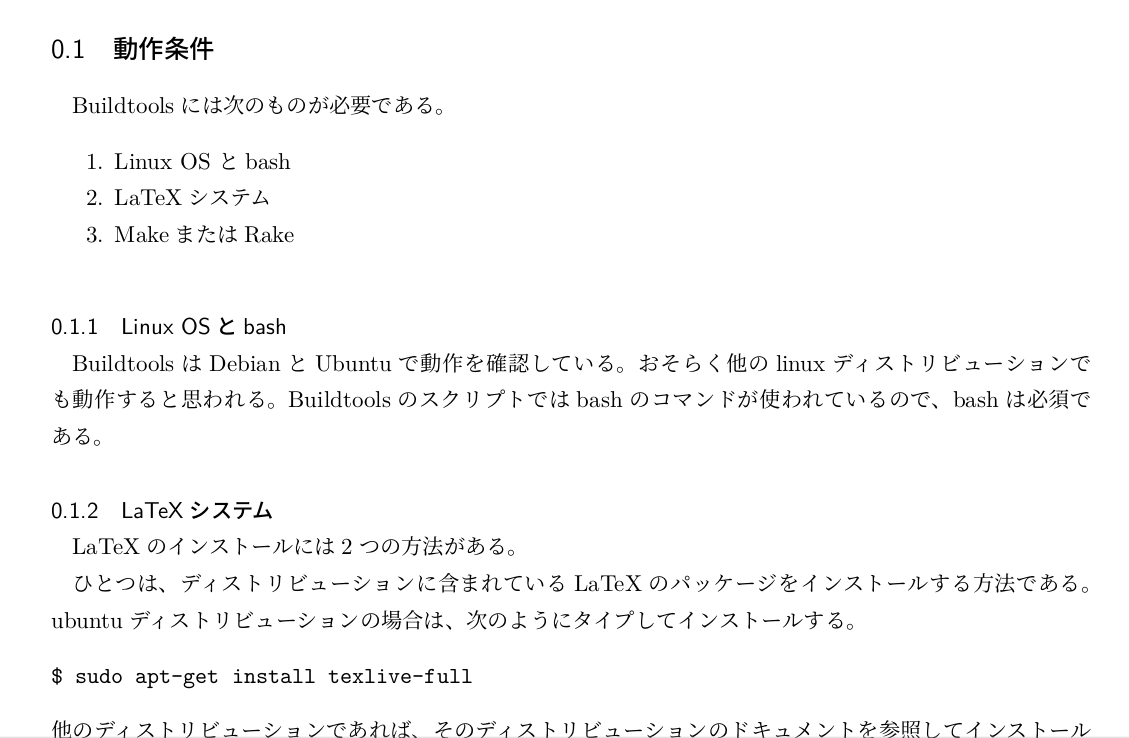
\includegraphics[width=12cm]{test_installation.png}
\end{center}

Lb compiles a subfile with the option synctex on.
Therefore, if you open the source files, `\_build/test\_installation.tex' and `installation.tex' in this example, you can do forward search and backward search between the source and pdf.
If your use gedit and evince, backward search works by clicking left button with pressing down CTRL key, but forward search from `installation.tex' doesn't work.
If you want to do it, add the following line at the beginning of the subfile.
\begin{verbatim}
% mainfile: _build/test_installation.tex
\end{verbatim}
However, forward search isn't used so often compared to backward search.
Adding the line above is usually unnecessary.


\section{プリプロセッシング}
  ときにはlatexソースファイルをコンパイルする前に何かしておきたい、ということがあるかもしれない。
例えば、
\begin{itemize}
\item gnuplotなどのプログラムを使って画像ファイルを生成したい
\item pandocを使ってlatexソースファイルを自動生成したい
\end{itemize}

このチュートリアルではプリプロセッサとしてpandocを使う方法を紹介したい。
pandocは文書コンバータである。
markdown、latex、html、pdfなど多くの種類の文書を変換することができる。
このチュートリアルでは、Buildtoolsのソースファイルの中にある「Readme.ja.md」を「readme.tex」というlatexソースファイルに変換してみる。

たいていのディストリビューションではpandocパッケージが備わっているので、インストールは簡単である。
例えばubuntuでは
\begin{verbatim}
$ sudo apt-get install pandoc
\end{verbatim}
でインストールできる。

readme.texを生成するには次のようにタイプする。
\begin{verbatim}
$ pandoc -o readme.tex ../Readme.ja.md
\end{verbatim}

この他に2つほどmain.texとhelper.texに変更を加える必要がある。
まず、{\textbackslash}inputコマンドを用いてreadme.texを取り込む命令をmain.texの最後に記述する。
\begin{verbatim}
\documentclass{article}
\input{helper.tex}
 ... ...
 ... ...
\section{Make tarball}
  \input{tarball.tex}
\input{readme.tex}
\end{document}
\end{verbatim}
更に、8行目の{\textbackslash}tableofcontentsをアンコメントしてコマンドが利くようにしよう。
\begin{verbatim}
 ... ...
\maketitle
% If you want a table of contents here, uncomment the following
 line.
\tableofcontents
 ... ...
\end{verbatim}

2番めは、{\textbackslash}tightlistのマクロを定義することが必要である。
Helper.texがその定義を書くのに最も適した場所である。
\begin{verbatim}
 ... ...
 ... ...
\providecommand{\tightlist}{%
  \setlength{\itemsep}{0pt}\setlength{\parskip}{0pt}}
 ... ...
 ... ...
\end{verbatim}
このコードは\url{https://github.com/jgm/pandoc-templates/blob/master/default.latex}から引用したものである。

rakeを使ってコンパイルする。
\begin{verbatim}
$ rake
\end{verbatim}

\begin{center}
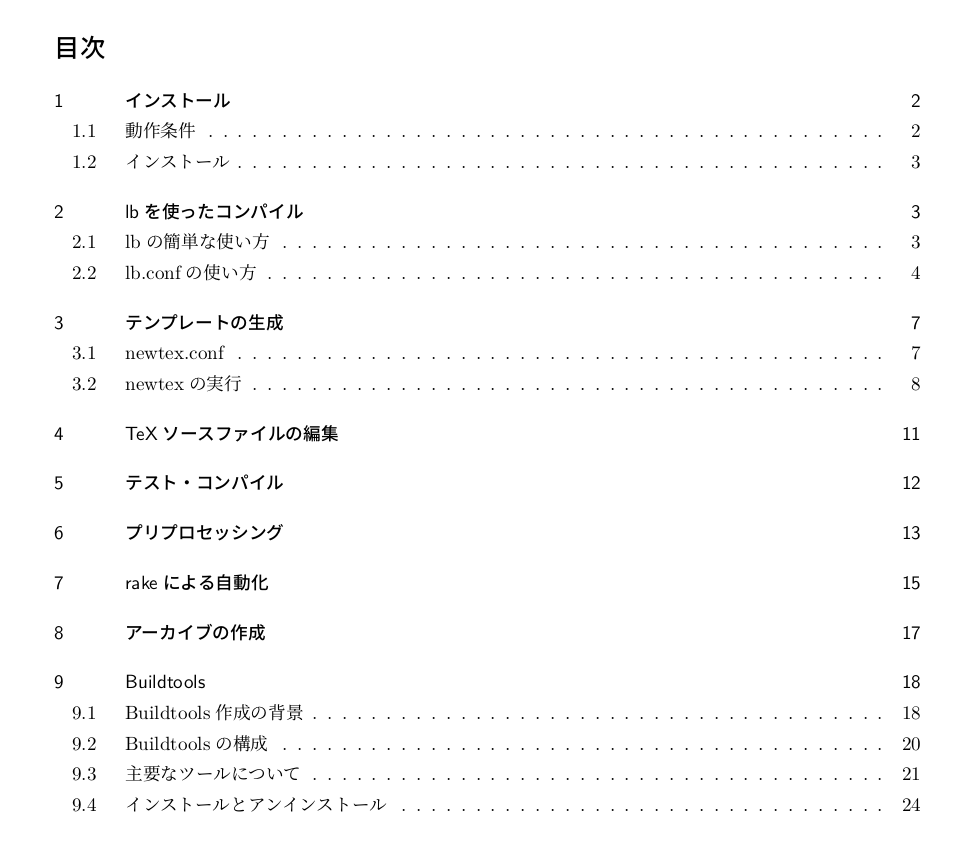
\includegraphics[width=12cm]{tableofcontents.png}
\end{center}

これで、目次にセクション9、そして「Readme.ja.md」の内容が表示された。

このセクションではpandocを手動で走らせた。
もしも、Readme.ja.md がアップグレードされたならば、再びpandocを実行しなければならない。
それは面倒なことであり、本来自動化されるべきことである。
ひとつの方法はRakefileを変更してrakeがコンパイル前に自動的にプリプロセッシングするようにすることである。
次のセクションでその方法を説明する。


\section{rakeによる自動化}
  rakeはmakeに似たビルド・ツールである。
Rakefileには、rakeがソースファイルをビルドする手順が書かれている。
Rakefileには任意のrubyコマンドを記述することができる。
したがって、そのビルドの過程が、たとえ複雑であってもそれを記述することが可能である。

newtexは自動的にRakefileを生成するが、プリプロセッシングが無ければ、そのままで十分使うことができる。
前セクションでは、readme.texを生成するためにpandocを用いたプリプロセッシングが行われた。
したがって、Rakefileを変更してpandocをその中に記述する必要がある。
以下のようにRakefileを変更する。
In the previous section, we used pandoc to generate readme.tex.
So, we need to modify Rakefile to put in pandoc.
Modify the Rakefile as follows.
\begin{verbatim}
require 'rake/clean'

# if readme.tex doesn't exist, generate it first.
# This is necessary because readme.tex is accessed by gfiles in
#  line 12.
if File.exist?("readme.tex") == false
  sh "pandoc -o readme.tex ../Readme.md"
end
# use Latex-BuildTools
@tex_files = (`tfiles -a` + `tfiles -p`).split("\n")
@tex_files <<= "readme.tex"
@graphic_files = []
@tex_files.each do |file|
  @graphic_files += `gfiles #{file}`.split("\n")
end

task default: "チュートリアル.pdf"

file "チュートリアル.pdf" => "_build/main.pdf" do
  sh "cp _build/main.pdf チュートリアル.pdf"
end

file "_build/main.pdf" => (@tex_files+@graphic_files) do
  sh "lb main.tex"
end

file "readme.tex" => "../Readme.ja.md" do
  sh "pandoc -o readme.tex ../Readme.ja.md"
end

CLEAN << "_build"
task :clean

task :ar do
  sh "arl main.tex"
  sh "tar -rf main.tar Rakefile"
  sh "gzip main.tar"
  sh "mv main.tar.gz チュートリアル.tar.gz"
end

task :zip do
  sh "arl -z main.tex"
  sh "zip main.zip Rakefile"
  sh "mv main.zip チュートリアル.zip"
end\end{verbatim}

この変更のおかげで、pandocを手動で走らせる必要はなくなった。
やらなければいけないのは、ただ単に「rake」とタイプするだけである。

rubyとrakeに関するウェブサイトはいくつかある。
例えば、
\begin{itemize}
\item \url{https://www.ruby-lang.org/en/}
\item \url{http://rubylearning.com/}
\item \url{https://ruby.github.io/rake/}
\end{itemize}
がその主なもので、参照してほしい。

\section{アーカイブの作成}
  You might want to distribute your source files.
Then, you need to archive them.
The script `arl' looks for the subfiles and the graphics files included by the rootfile, and archive them.
\begin{itemize}
\item If -g option is given, it makes gzip compressed tarball.
\item If -b option is given, it makes bzip2 compressed tarball.
\item If -z option is given, it makes zip file.
\item If no option is given, it makes non-compressed tarball.
\end{itemize}

If some latex source files are generated by preprocessing, you need to generate them before running arl.
\begin{verbatim}
$ arl
$ tar -tf main.tar
main.tex
edit_tex_files.tex
generate_templates.tex
installation.tex
lb.tex
preprocessing.tex
rake.tex
readme.tex
tarball.tex
test_compile.tex
helper.tex
Tutorial_1.png
Tutorial_2.png
hellolatex.png
tableofcontents.png
test_installation.png
\end{verbatim}

Rakefile needs to be added to the tarball.
\begin{verbatim}
$ tar -rf main.tar Rakefile
\end{verbatim}
Then, compress it into gzip.
\begin{verbatim}
$ gzip main.tar
\end{verbatim}

The procedure above is already written in the Rakefile.
Type `rake ar', then rake makes a tarball.
\begin{verbatim}
$ rm main.tar.gz
$ rake ar
arl main.tex
tar -rf main.tar Rakefile
gzip main.tar
mv main.tar.gz Tutorial.tar.gz
\end{verbatim}
Now the name of the tarball is `Tutorial.tar.gz'.

If you want to make a zip file, type `rake zip'.

The tutorial finishes at this section.
Next section is the copy of Readme.md in Buildtools source files.
It describes the background of Buildtools and features of each script.

\end{document}
\end{verbatim}
最初の行はドキュメントクラスの指定で、newtex.confのdovumentclassキーの値が引数になっている。
2番めの行ではhelper.texを取り込むinputコマンドが書かれている。
helper.texは\verb|\usepackage|コマンドでパッケージを取り込んだり、\verb|\newcommand|コマンドでマクロを定義するなどの役割がある。
プリアンブルの記述のほとんどはhelper.texに書かれている。
ユーザが自分専用のhelper.texを作っておくのは、良い考えである。
というのは、同じプリアンブルをいろいろな文書に使い回すことが多いからである。
自分専用helper.texを持っているユーザはこのテンプレートを上書きすると良い。

4行目は書き直しが必要である。
例えば、
\begin{verbatim}
\author{関谷 敏雄}
\end{verbatim}
のように。
`{\textbackslash}date'、`{\textbackslash}thanks'、abstract環境などを必要に応じて付け加えて良い。
また、目次が必要であれば、8行目のハッシュマークを外して、アンコメントする。
残りの行は、セクションとそのセクションの内容を記述したサブファイルを取り込むための{\textbackslash}inputコマンドである。

Rakefileはrakeに対する指示を書いたファイルである。
当面はこれを書き換える必要はない。
テンプレートをそのまま使い、rakeを実行してみよう。
\begin{verbatim}
$ rake
 ... ...
 ... ...
$ ls
Makefile            generate_templates.tex  preprocessing.tex
Rakefile            helper.tex              rake.tex
_build              installation.tex        tarball.tex
cover.tex           lb.conf                 test_compile.tex
edit_tex_files.tex  lb.tex                  チュートリアル.pdf
gecko.png           main.tex
$ ls _build
main.aux          main.fls  main.out
main.fdb_latexmk  main.log  main.pdf
$ evince Tutorial.pdf
\end{verbatim}
rakeはlbを起動してmain.texをコンパイルし、その後「\_build/main.pdf」を「チュートリアル.pdf」にコピーする。
Evinceは「チュートリアル.pdf」を次のように表示してくれる。
\begin{center}
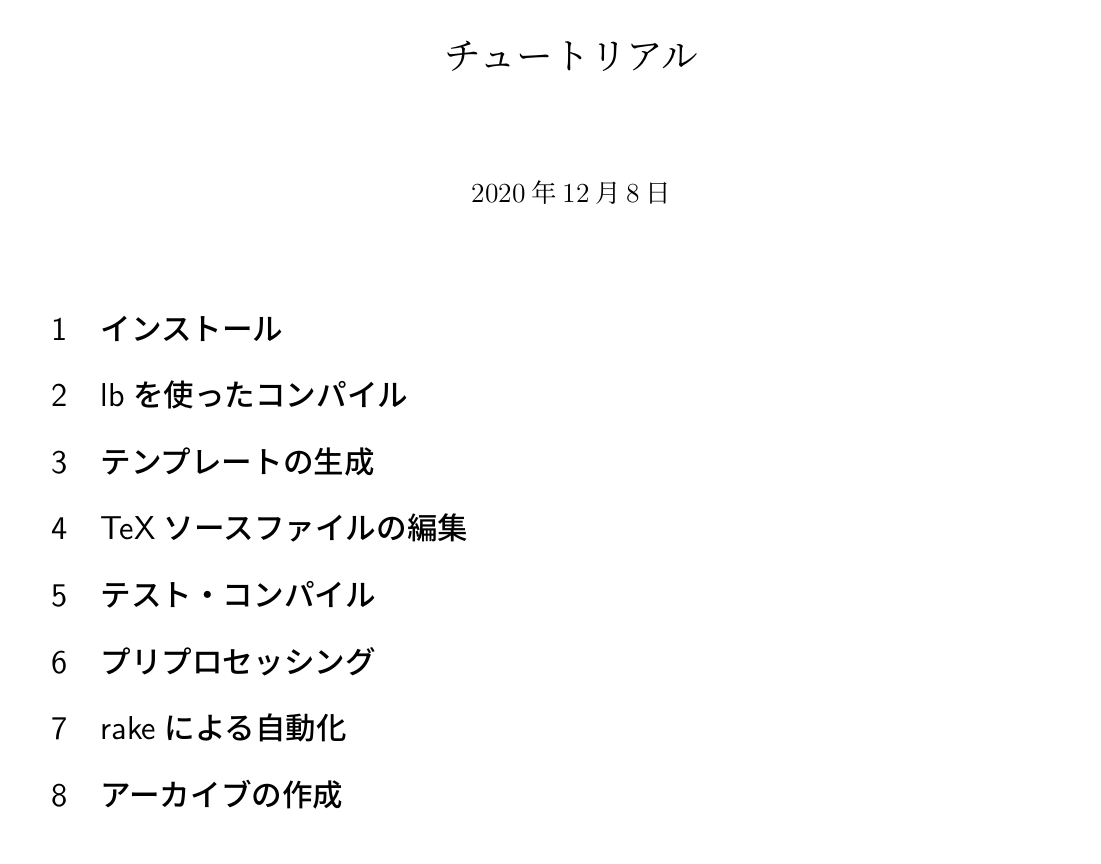
\includegraphics[width=12cm]{Tutorial_1.png}
\end{center}


\section{TeXソースファイルの編集}
  main.texには8つのセクションとそれに対応するサブファイルを取り込む{\textbackslash}inputコマンドが書かれている。
それぞれのサブファイルはテンプレートとして生成された直後は空のファイルである。
そのサブファイルの編集が文書作成の主要な作業になり、作成にかかる時間の大部分がそれに当てられる。

ところで、セクションの編集の途中でも、そこまでをpdfにするとどうなるかを見たいことがあるだろう。
そのためのコンパイルをテスト・コンパイルという。
多くの場合、編集とテスト・コンパイルの間を何回も行ったり来たりしながら、文書作成が進むものである。

もしも、文書がさほど大きくないならば、rakeを用いるのがテスト・コンパイルには最も良い。
というのは、さほどコンパイル時間もかからず、文書全体のpdfを見ることができるからである。
このチュートリアルは、どちらかといえば小さい文書であるから、rakeをテスト・コンパイルに用いるのが良い。

さて、最初のセクションを編集する代わりに、ソースファイル「installation.tex」をコピーしよう。
\begin{verbatim}
\subsection{動作条件}
Buildtoolsには次のものが必要である。
\begin{enumerate}
\item Linux OS とbash
\item LaTeXシステム
\item MakeまたはRake
\end{enumerate}
 ... ...
 ... ...
\end{verbatim}
コピーがすんだら、下記のようにタイプしてpdfを見てみよう。
\begin{verbatim}
$ rake
$ evince チュートリアル.pdf
\end{verbatim}

\begin{center}
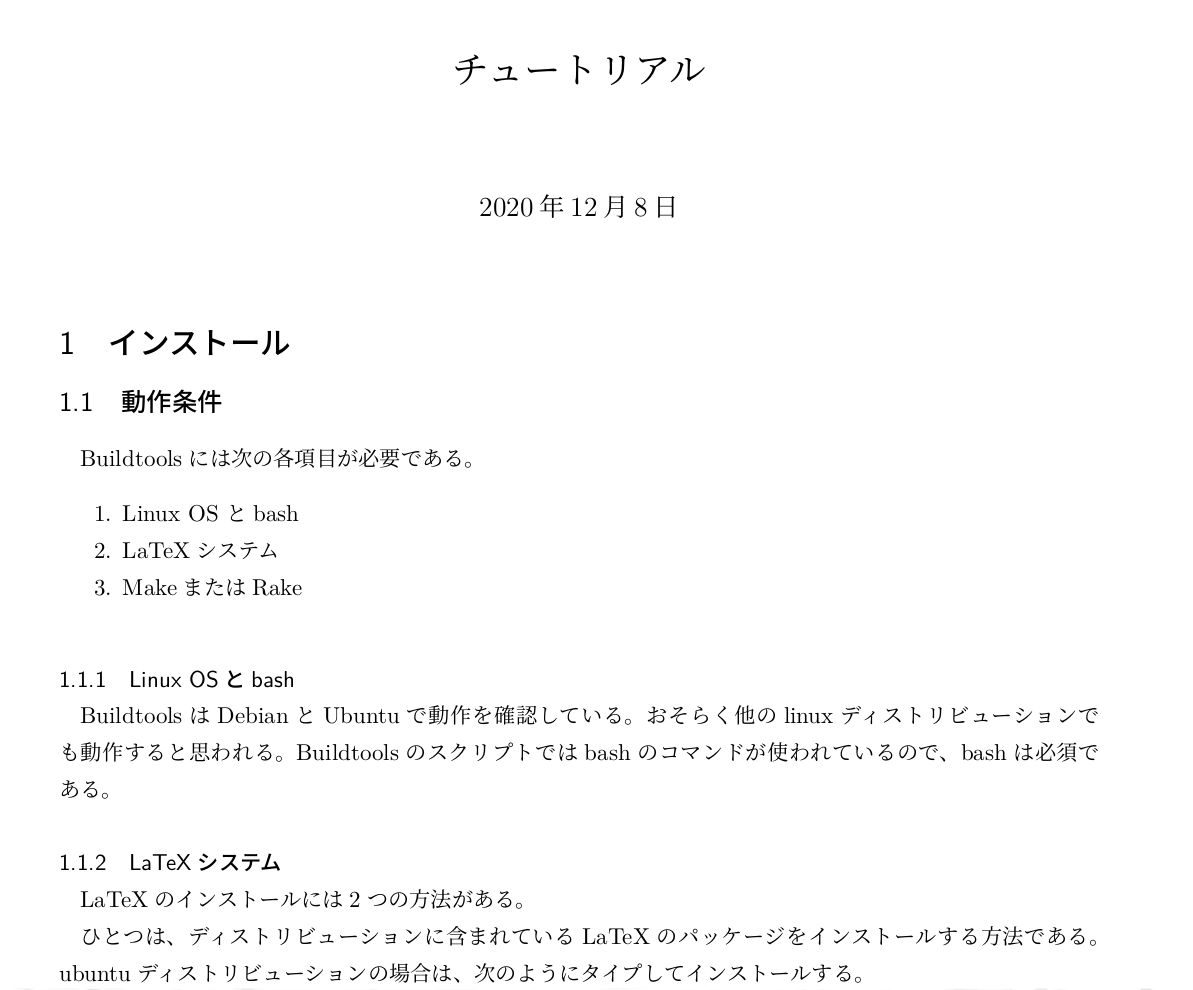
\includegraphics[width=12cm]{Tutorial_2.png}
\end{center}

\section{テスト・コンパイル}
  If you make a big document, for example a book which has more than 100 pages, then using rake is not a good way to test-compile.
The bigger the dicument is, the longer time the compiling takes.

It is a better way to use `lb' to test-compile a subfile separately.
Lb makes a temporary rootfile which includes only the subfile and compile it once.
The advantage of this way is very quick to compile.
However, it has disadvantages.
It only compiles the subfile, so the pdf you get is not a finished document.
It compiles once, so cross-reference doesn't work at all.
It is difficult to say which is better.
it depends on the size of your document.
If it is very big, use lb to test-compile separately.

In this section, I want to show you how to use lb to test-compile a subfile.
This document `Tutorial' is not big, but it's OK.
This is an example to show how to use lb.

Type the following.
\begin{verbatim}
$ lb installation
\end{verbatim}
The argument is a subfile.
The suffix can be left out.
Then, lb makes a temporary rootfile `\_build/test\_installation.tex'.
Its preamble is a copy of the preamble in the original rootfile.
It has {\textbackslash}input command and includes the subfile `installation.tex'.
Lb compiles `\_build/test\_installation.tex' and run the previewer specified in `lb.conf' to show the pdf.
\begin{center}
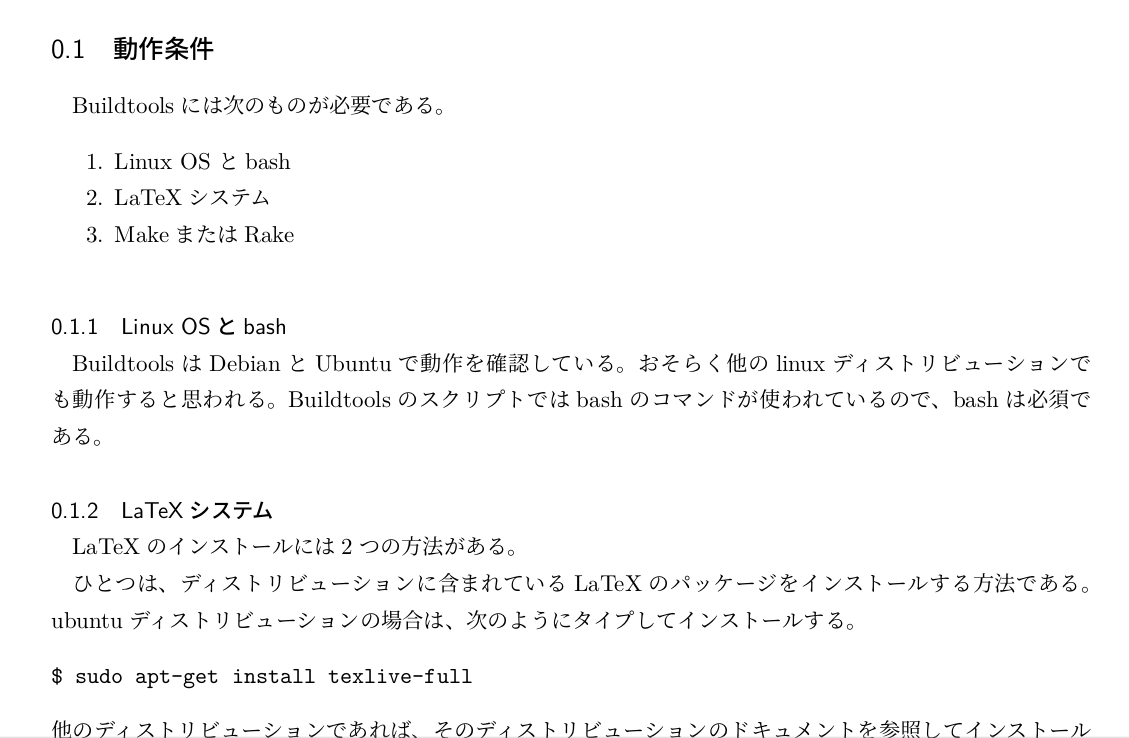
\includegraphics[width=12cm]{test_installation.png}
\end{center}

Lb compiles a subfile with the option synctex on.
Therefore, if you open the source files, `\_build/test\_installation.tex' and `installation.tex' in this example, you can do forward search and backward search between the source and pdf.
If your use gedit and evince, backward search works by clicking left button with pressing down CTRL key, but forward search from `installation.tex' doesn't work.
If you want to do it, add the following line at the beginning of the subfile.
\begin{verbatim}
% mainfile: _build/test_installation.tex
\end{verbatim}
However, forward search isn't used so often compared to backward search.
Adding the line above is usually unnecessary.


\section{プリプロセッシング}
  ときにはlatexソースファイルをコンパイルする前に何かしておきたい、ということがあるかもしれない。
例えば、
\begin{itemize}
\item gnuplotなどのプログラムを使って画像ファイルを生成したい
\item pandocを使ってlatexソースファイルを自動生成したい
\end{itemize}

このチュートリアルではプリプロセッサとしてpandocを使う方法を紹介したい。
pandocは文書コンバータである。
markdown、latex、html、pdfなど多くの種類の文書を変換することができる。
このチュートリアルでは、Buildtoolsのソースファイルの中にある「Readme.ja.md」を「readme.tex」というlatexソースファイルに変換してみる。

たいていのディストリビューションではpandocパッケージが備わっているので、インストールは簡単である。
例えばubuntuでは
\begin{verbatim}
$ sudo apt-get install pandoc
\end{verbatim}
でインストールできる。

readme.texを生成するには次のようにタイプする。
\begin{verbatim}
$ pandoc -o readme.tex ../Readme.ja.md
\end{verbatim}

この他に2つほどmain.texとhelper.texに変更を加える必要がある。
まず、{\textbackslash}inputコマンドを用いてreadme.texを取り込む命令をmain.texの最後に記述する。
\begin{verbatim}
\documentclass{article}
% helper.tex

% You need to rewrite this file to fit your build environment.

% Notice
% The driver of graphicx package is luatex.
% If you use another engine, then you need to rewrite it to your driver.
% For example, if you use pdflatex, then the driver is pdftex.

% Packages
\usepackage{amsmath,amssymb}
\usepackage[luatex]{graphicx}
\usepackage{tikz}
\usetikzlibrary{calc}
\usetikzlibrary{topaths}
\usetikzlibrary{plotmarks}
\usetikzlibrary{intersections}
\usetikzlibrary{arrows,decorations.pathmorphing,backgrounds,positioning,fit,petri}
\usetikzlibrary{arrows.meta}
\usetikzlibrary{3d}

\usepackage{fancybox}
\usepackage{booktabs}

\usepackage[margin=2.4cm]{geometry}

\usepackage[colorlinks=true,linkcolor=black]{hyperref}

% Sample macro.
%\newcommand{\solution}{\begin{flushleft}\textbf{Solution:}\end{flushleft}}
%\newcommand{\proof}{\begin{flushleft}\textbf{Proof}\end{flushleft}}
%\newcommand{\qed}{\begin{flushright}\textbf{q. e. d.}\end{flushright}}
%\newcommand{\answer}[1]{\begin{flushleft}\textbf{Exercise~\ref{#1}}\end{flushleft}}

% Theorem environment.
%\newtheorem{theorem}{Theorem}[section]
%\newtheorem{lemma}{Lemma}[section]
%\newtheorem{corollary}{Corollary}[section]
%\newtheorem{definition}{Definition}[section]
%\newtheorem{example}{Example}[section]
%\newtheorem{exercise}{Exercise}[section]

 ... ...
 ... ...
\section{Make tarball}
  You might want to distribute your source files.
Then, you need to archive them.
The script `arl' looks for the subfiles and the graphics files included by the rootfile, and archive them.
\begin{itemize}
\item If -g option is given, it makes gzip compressed tarball.
\item If -b option is given, it makes bzip2 compressed tarball.
\item If -z option is given, it makes zip file.
\item If no option is given, it makes non-compressed tarball.
\end{itemize}

If some latex source files are generated by preprocessing, you need to generate them before running arl.
\begin{verbatim}
$ arl
$ tar -tf main.tar
main.tex
edit_tex_files.tex
generate_templates.tex
installation.tex
lb.tex
preprocessing.tex
rake.tex
readme.tex
tarball.tex
test_compile.tex
helper.tex
Tutorial_1.png
Tutorial_2.png
hellolatex.png
tableofcontents.png
test_installation.png
\end{verbatim}

Rakefile needs to be added to the tarball.
\begin{verbatim}
$ tar -rf main.tar Rakefile
\end{verbatim}
Then, compress it into gzip.
\begin{verbatim}
$ gzip main.tar
\end{verbatim}

The procedure above is already written in the Rakefile.
Type `rake ar', then rake makes a tarball.
\begin{verbatim}
$ rm main.tar.gz
$ rake ar
arl main.tex
tar -rf main.tar Rakefile
gzip main.tar
mv main.tar.gz Tutorial.tar.gz
\end{verbatim}
Now the name of the tarball is `Tutorial.tar.gz'.

If you want to make a zip file, type `rake zip'.

The tutorial finishes at this section.
Next section is the copy of Readme.md in Buildtools source files.
It describes the background of Buildtools and features of each script.

\hypertarget{buildtools}{%
\section{Buildtools}\label{buildtools}}

\hypertarget{the-background-of-buildtools}{%
\subsection{The background of
Buildtools}\label{the-background-of-buildtools}}

\hypertarget{buildtools-is-a-part-of-latextools}{%
\paragraph{Buildtools is a part of
Latextools}\label{buildtools-is-a-part-of-latextools}}

If you make a long document, for example, a book with more than a
hundred pages, you need to consider various things which isn't necessary
in creating a short document.

\begin{itemize}
\tightlist
\item
  Divide the source file into small parts
\item
  Compile each parts independently
\item
  Replace something with another in the whole document
\item
  Preprocessing (processes before compiling latex source files)
\end{itemize}

Latextools support these things and it includes two parts.

\begin{itemize}
\tightlist
\item
  Buildtools. It is tools which support creating templates of source
  files, building and partial compiling.
\item
  Substools. It is tools which perform replacements in the whole
  document.
\end{itemize}

Buildtools is a part of Latextools and also a core tools in it. This
document describes Buildtools only.

\hypertarget{dividing-a-source-file}{%
\paragraph{Dividing a source file}\label{dividing-a-source-file}}

Latex source files are simply called source files here. It is not
appropriate to write a long document into a single source file. Because,
bigger the file, much more difficult to edit it. To solve this, the
document will be divided into some parts. Usually, they consist of a
file containing \texttt{\textbackslash{}begin\{document\}} and
\texttt{\textbackslash{}end\{document\}} and the other files called by
the file with \texttt{\textbackslash{}include} or
\texttt{\textbackslash{}input} command. The former file is called
rootfile and the latter files are called subfiles. There is a difference
between \texttt{\textbackslash{}include} and
\texttt{\textbackslash{}input} though both are commands to include
subfiles.

\begin{itemize}
\item
  \texttt{\textbackslash{}include} can't be nested. it can be described
  only in the body, which means the part between
  \texttt{\textbackslash{}begin\{document\}} and
  \texttt{\textbackslash{}end\{document\}}.
  \texttt{\textbackslash{}includeonly}, which must be in the preamble,
  specifies a list of files to include by the
  \texttt{\textbackslash{}include} command. The files in the list are
  included by \texttt{\textbackslash{}include} command, and files out of
  the list aren't included even if it is an argument of
  \texttt{\textbackslash{}include} command.
  \texttt{\textbackslash{}include} command issues
  \texttt{\textbackslash{}clearpage} command before and after including
  the file.
\item
  \texttt{\textbackslash{}input} command simply include files. It
  doesn't issue \texttt{\textbackslash{}clearpage} command. This command
  can be nested.
\end{itemize}

It is called build to make a document by compiling. It includes not only
the compilation with latex but also the preprocessing, such as the image
generation by gnuplot or tikz graph generation with data. It is finally
completed by the compilation of the rootfile.

There are several programs to compile LaTeX source files, and they are
called engines. Buildtools supports latex, platex, pdflatex, xelatex and
lualate as engines.

The bigger the document to compile is, the longer the time needs. Even
if you change a small part of the document, it needs the same time as
the big change. You often need to compile to check how the pdf document
looks like, which is sometimes called test, it needs long time in each
compilation. The bigger the document is, the more serious the problem
is. So, it has been thought up to compile a subfile itself without
rootfile or other subfiles.

\begin{itemize}
\tightlist
\item
  Comment out the files in the argument list of
  \texttt{\textbackslash{}includeonly} command which you don't want to
  compile.
\item
  Use subfiles package.
\end{itemize}

Subfiles package is nice and many people recommend it. However, you need
to include the package and use its command appropriately. Naturally, it
is not the matter compared with the compilation time above.

Another way is to add an specific preamble to compile a subfile without
any other files. More specifically, the subfile is put between ``the
text from \texttt{\textbackslash{}documentclass} to
\texttt{\textbackslash{}begin\{document\}}'' and
``\texttt{\textbackslash{}end\{document\}}''. On that occasion, the
subfile itself isn't changed, but another file, which contains the
preamble, \texttt{\textbackslash{}end\{document\}} and
\texttt{\textbackslash{}input} command, is made. The
\texttt{\textbackslash{}input} command reads the subfile. The file newly
made is called ``temporary rootfile''. On the other hand, the rootfile
is sometimes called " original rootfile". The preamble in the temporary
rootfile is a copy of the preamble in the original rootfile. The good
point of this way is:

\begin{itemize}
\tightlist
\item
  There's no need to include any packages or put any special commands.
\item
  Therefore, users don't need to install any packages when the source
  file is distributed.
\end{itemize}

The point is subfile can be compiled separately without any modification
in the source files. The generation of the temporary rootfile is the
only necessary. Buildtools has \texttt{ttex} shell script to do that.

\hypertarget{repeating-compiling}{%
\paragraph{Repeating compiling}\label{repeating-compiling}}

It often needs to compile source files two times or more because of the
cross-reference. The repeating times are maybe two or three (or more),
but I don't know the details. However, there's a great software that
calculate the repeating times automatically. It is latexmk. Latexmk make
the build very easy. Buildtools uses latexmk to compile rootfiles.

\hypertarget{build-directory}{%
\paragraph{Build directory}\label{build-directory}}

Some people might complain about latex because it generates various of
auxiliary files and log files. If you make a build directory and put all
the generated files into it, the source directory can be kept clean. One
of such program is cluttex and it is recommended to people who like
cleanliness.

Buildtools makes a temporary directory, which is also called build
directory, and put all the temporary files and generated document. The
default name of the directory is \texttt{\_build}. It makes the source
directory keep clean. If you want to see log or auxiliary files, search
the build directory for them. It's very simple. Although it is
superfluous to say so, meson build system which is very popular as a C
build tool also uses build directory. This shows us that separating
build directory from source directory is very easy to understand.

Lb, one of the tools in Buildtools, generate a final pdf document in the
build directory. However, many users probably want to put it in the
source directory. It is a natural idea. If you want to do so, use make
or rake.

Rake is a similar program to make. Its advantage is using ruby language
in the Rakefile, which is the script file of rake. Because ruby language
is very strong and flexible, the script file can be readable and
structured.

To get back to the subject how to put a final pdf document in the source
directory, you just write a cp command in your Makefile or Rakefile to
copy the pdf document under the build directory into source directory.
Furthermore, the advantage to use make or rake is that it's possible to
specify preprocessing code in the Makefile or Rakefile. Because
preprocessing depends on the document and what tools the user choose,
it's difficult for Buildtools to cover the preprocessing. Compared with
that, Makefile or Rakefile are really flexible so that you can write
your own preprocessing in it.

It is recommended that users should use make or rake with Buildtools.

\hypertarget{combination-with-texworks}{%
\paragraph{combination with Texworks}\label{combination-with-texworks}}

Lb, one of the tools in Buildtools, can either compile a rootfile or
test-compile a subfile. If you specify it into proccessing tools in the
texworks dialog, you can run lb from texworks and it's so convenient.
Click edit, preference, then typesetting tab. Click plus button in the
processing tools part, then put \texttt{lb}, \texttt{lb},
\texttt{\$fullname} in name, program and arguments box respectively.
Once you set it, you can compile a rootfile or test-compile a subfile by
clicking on the typesetting icon (green triangle icon).

\hypertarget{buildtools-structure}{%
\subsection{Buildtools structure}\label{buildtools-structure}}

Buildtools is made up of the following five parts.

\begin{itemize}
\tightlist
\item
  \texttt{newtex}: It generates source file templates. This is used at
  the beginning of making documents.
\item
  \texttt{lb}: It calls latexmk or ttex to compile source files.
\item
  \texttt{arl}: It makes an archive file.
\item
  installer
\item
  a group of utilities. They are used by the tools above.
\end{itemize}

The following shows the steps to build documents.

\begin{enumerate}
\def\labelenumi{\arabic{enumi}.}
\tightlist
\item
  Make the structure, especially the chapters/sections, of the
  document..
\item
  Run newtex and make folders and templates of the document.
\item
  Modify the templates of Makefile, Rakefile, cover page (cover.tex) and
  preamble (cover.tex) if necessary.
\item
  Write the body of the document and test-compile.
\item
  If necessary, make script files for the preprocessing.
\item
  Compile the rootfile to generate the final pdf document.
\end{enumerate}

The step three to five above are usually repeated and the process is not
necessarily in the order above.

\hypertarget{main-tools}{%
\subsection{Main tools}\label{main-tools}}

Each tool shows its help message if it is run with \texttt{-\/-help}
option. For example, newtex shows the following message.

\begin{verbatim}
$ newtex --help
Usage:
  newtex --help
    Show this message.
  Newtex.conf needs to be edited before running newtex.
  newtex
    A directory is made and some template files are generated under the directory.
\end{verbatim}

The document of each tool is:

\begin{itemize}
\tightlist
\item
  The help message shown by each command with \texttt{-\/-help} option.
\item
  The description below in this document.
\end{itemize}

No other document exists. If you want to know more, see the source code.
All the tools in Buildtools are shell scripts. If you are familiar to
shell scripts, you can easily understand them because they are short.

\hypertarget{newtex}{%
\paragraph{newtex}\label{newtex}}

\begin{verbatim}
$ newtex
\end{verbatim}

Newtex is used when you make a new latex document. irst, decide the
structure and chapters and make \texttt{newtex.conf} in advance. This
script makes a directory and generates template files according to
\texttt{newtex.conf}.

\begin{enumerate}
\def\labelenumi{\arabic{enumi}.}
\tightlist
\item
  There is \texttt{newtex.conf} file in the Buildtools source files.
  Modify it to fit your environment and tex source files you will make.
\item
  Execute \texttt{newtex}. Then it make a directory which name is the
  same as \texttt{title} in \texttt{newtex.conf}. However, the space
  characters in the value of \texttt{title} is converted to underscore
  in the name of the directory. The script also generates template files
  under the directory.
\end{enumerate}

\hypertarget{lb}{%
\paragraph{lb}\label{lb}}

\begin{verbatim}
$ lb [LaTeXfile]
\end{verbatim}

If the argument is left out, \texttt{lb} behaves as if \texttt{main.tex}
is specified as an argument. \texttt{Lb} is a script to build LaTeX
source files and you usually don't need anything except it.

\begin{itemize}
\tightlist
\item
  If the argument is rootfile, then \texttt{lb} compiles it with
  \texttt{latexmk}. If the argument is subfile, then \texttt{lb} runs
  \texttt{ttex} specifying the subfile as an argument.
\item
  If the argument is rootfile, \texttt{lb} compiles it without synctex.
\item
  If the argument is subfile, \texttt{lb} runs \texttt{ttex} and
  \texttt{ttex} compiles the subfile with synctex. After compilation,
  \texttt{lb} runs previewer specified in \texttt{lb.conf}.
\item
  If there exists \texttt{lb.conf} in the current directory (it usually
  contains the rootfile), \texttt{lb} reads it and initialize some
  variables.
\item
  If the variable \texttt{engine} in \texttt{lb.conf} is null string,
  then \texttt{lb} guesses an appropriate engine by itself. However, it
  is recommended that you should specify the engine in \texttt{lb.conf}.
\end{itemize}

You can specify the default values in \texttt{lb.conf} to initialize
some variables.

\begin{verbatim}
rootfile=main.tex
builddir=_build
engine=
latex_option=-halt-on-error
preview=texworks
\end{verbatim}

\begin{itemize}
\tightlist
\item
  \texttt{rootfile} is the name of the rootfile. If you specify the name
  of the rootfile as an argument to \texttt{lb}, then the argument takes
  precedence.
\item
  \texttt{builddir} is the name of the build directory. Auxiliary files
  and output files are put in the build directory. If the argument of
  \texttt{lb} is a subfile, then the temporary rootfile is also put in
  the build directory. If \texttt{builddir} is empty, then no temporary
  directory is generated and the source file directory becomes a build
  directory.
\item
  \texttt{engine} is the name of a latex engine. \texttt{latex},
  \texttt{platex}, \texttt{pdflatex}, \texttt{xelatex} and
  \texttt{lualatex} can be specified. Other engines are not supported.
\item
  \texttt{latex\_option} is a list of options to specify as an argument
  to the engine through \texttt{latexmk}. \texttt{-output-directory} is
  automatically given to \texttt{latexmk} by \texttt{lb} even if
  \texttt{lb.conf}doesn't exist.
\item
  \texttt{preview} is the name of a pdf previewer to show the document.
  It is run only if the argument of \texttt{lb} is a subfile.
\end{itemize}

\hypertarget{arl}{%
\paragraph{arl}\label{arl}}

\$ arl {[}-b\textbar{}-g\textbar{}-z{]} {[}rootfile{]}

The name \texttt{arl} comes from ``ARchive LaTeX files''. It searches
the rootfile for its related files (refer the following) and make an
archive file. If the argument is left out, then it runs as if
\texttt{main.tex} is specified as an argument.

\begin{itemize}
\tightlist
\item
  If there are preprocessing programs, you need to execute them before
  running arl.
\item
  Arl archives the latex source files and the graphic files included by
  \texttt{\textbackslash{}includegraphics} command.
\item
  Therefore, \texttt{Makefile} or the preprocessing script files are not
  archived.
\end{itemize}

It is a good way to make a target (for example, its name is `ar') in
Makefile and write a recipe to add Makefile and the preprocessing files
into the archive file made by \texttt{arl}. You can do the same thing
with Rakefile.

There are options \texttt{-g}, \texttt{-b} and \texttt{-z} to compress
the archive file into \texttt{tar.gz}, \texttt{tar.bz2} and \texttt{zip}
file respectively. If no option is given, \texttt{arl} just make a
tarball without compression.

\hypertarget{utilities}{%
\paragraph{Utilities}\label{utilities}}

You don't need to read this subsection except maintaining the scripts.

\begin{verbatim}
$ srf subfile
\end{verbatim}

This script \texttt{srf} searches for the rootfile of the given subfile
and outputs its absolute path. \texttt{srf} comes from ``Search for Root
File''.

\begin{verbatim}
$ tfiles [-p|-a|-i] [rootfile]
\end{verbatim}

It outputs a list of subfiles of the given rootfile. If the argument is
left out, then it is run as if \texttt{main.tex} is specified as an
argument.

\begin{itemize}
\tightlist
\item
  No option: It outputs a list of subfiles, specified from
  \texttt{\textbackslash{}begin\{document\}} to
  \texttt{\textbackslash{}end\{document\}}. They are the arguments of
  \texttt{\textbackslash{}include} or \texttt{\textbackslash{}input}
  command.
\item
  \texttt{-p}: It outputs a list of subfiles specified with the
  \texttt{\textbackslash{}input} commands in the preamble of the
  rootfile.
\item
  \texttt{-a}: It outputs a list, outputted with no option, and the
  rootfile itself.
\item
  \texttt{-i}: It outputs a list of subfiles specified with both
  \texttt{\textbackslash{}include} and
  \texttt{\textbackslash{}includeonly} command.
\end{itemize}

The files in the list are separated with new lines.

\begin{verbatim}
$ tftype [-r|-s|-q] files ...
\end{verbatim}

It outputs or returns the type of the given latex files.

\begin{itemize}
\tightlist
\item
  \texttt{-r}: It outputs rootfiles which is in the argument files. If
  no options are given, It behaves as if this option is specified.
\item
  \texttt{-s}: It outputs subfiles which is in the argument files.
\item
  \texttt{-q}: It doesn't output anything. The number of the argument
  must be one. It returns an exit status code of the file type. If the
  code is 0 or 1, then the file is a rootfile or subfile respectively.
  Otherwise an error happens.
\end{itemize}

Using \texttt{-q} option is the most common.

\begin{verbatim}
$ gfiles files ...
\end{verbatim}

The argument is a list of latex source files. It outputs graphic files
which are included by \texttt{\textbackslash{}includegraphics} commands
in the given files.

\begin{verbatim}
$ ltxengine rootfile
\end{verbatim}

It guesses a latex engine to compile the rootfile, although it is
recommended that the engine should be specified by the user. For
example,

\begin{verbatim}
\usepackage[luatex]{graphicx}
\end{verbatim}

If this command exists in the preamble, it guesses that the engine is
probably lualatex.

\begin{verbatim}
$ ttex [-b builddir] -e latex_engine [-p dvipdf] [-v previewr] -r rootfile subfile
\end{verbatim}

It generates a temporary rootfile of the subfile and compile it. The
compilation is done only once. Therefore, no cross-reference is carried
out. This comes from the idea that \texttt{ttex} is a script for test to
see how the pdf file looks like and cross-reference is not so important.
The cross-reference to the other files doesn't work neither. This script
can be run directly on the command line, but usually it is called by
\texttt{lb}. The following shows the options.

\begin{itemize}
\tightlist
\item
  \texttt{-b}: Specify a build directory. The default is
  \texttt{\_build}.
\item
  \texttt{-e}: Specify a latex engine. There is no restriction on the
  engine, but it assumes that latex, platex, pdflatex, xelatex or
  lualatex is specified.
\item
  \texttt{-p}: Specify an application that translates dvi into pdf. This
  is used only when the engine is latex or platex, because they outputs
  a dvi file. The default is dvipdfmx. Other possible application is
  dvipdfm and dvipdf.
\item
  \texttt{-v}: Specify a pdf previewer like evince. If you edit the
  source file with texworks, it is a good idea to specify texworks here.
\item
  \texttt{-r}: Specify the original rootfile.
\end{itemize}

\hypertarget{installation-and-uninstallation}{%
\subsection{Installation and
uninstallation}\label{installation-and-uninstallation}}

\hypertarget{prerequisite}{%
\paragraph{Prerequisite}\label{prerequisite}}

\begin{itemize}
\item
  Linux and bash: It is tested on Debian and Ubuntu. However, it
  probably works on other linux distributions. Bash is required because
  this script includes bash commands.
\item
  LaTeX: There are two options to install LaTeX. One is installing the
  LaTeX applications provided by your distribution. The other is
  installing TexLive.
\item
  make or rake: These applications are not necessarily required to run
  the tools in Buildtools. However, it is recommended that they are used
  under the control of make or rake. You don't need to install both of
  them. Choose one which you like. Make is a traditional build tool
  originally aimed at C compiler. Rake is a build tool similar to make.
  It is one of the ruby application. The advantage to use rake is that
  you can put any ruby codes into Rakefile, which is the script file of
  rake. Generally speaking, Rakefile is easy to understand than
  Makefile.
\end{itemize}

\hypertarget{installation}{%
\paragraph{Installation}\label{installation}}

Use the script install.sh.

\begin{verbatim}
$ bash install.sh
\end{verbatim}

This script installs the executable files into \texttt{\$HOME/bin}.
Debian and Ubuntu adds the directory \texttt{\$HOME/bin} into
\texttt{PATH} environment variable if it exists at the login time. The
script makes the directory \texttt{\$HOME/bin} if it doesn't exist. In
that case, you need to re-login to put the directory into the
\texttt{PATH} environment variable. If you run \texttt{sudo} or
\texttt{su} to become the root user before the installation, the
executable files are put into \texttt{/user/local/bin}.

If your OS is debian, type the following to be the root user.

\begin{verbatim}
$ su -
# bash install.sh
\end{verbatim}

Or if it's ubuntu,

\begin{verbatim}
$ sudo bash install.sh
\end{verbatim}

\hypertarget{uninstallation}{%
\paragraph{Uninstallation}\label{uninstallation}}

Use the script uninstall.sh.

\begin{verbatim}
$ bash uninstall.sh
\end{verbatim}

If you run this as a user, the files under \texttt{\$HOME} are removed.
If you run this as a root, the files under \texttt{/usr/local} are
removed. If your OS is debian, type the following to be the root user.

\begin{verbatim}
$ su -
# bash uninstall.sh
\end{verbatim}

Or if it's ubuntu,

\begin{verbatim}
$ sudo bash uninstall.sh
\end{verbatim}

\hypertarget{licence}{%
\subsection{licence}\label{licence}}

Copyright (C) 2020 ToshioCP (Toshio Sekiya)

Buildtools is free software; you can redistribute it and/or modify it
under the terms of the GNU General Public License as published by the
Free Software Foundation; either version 3 of the License, or (at your
option) any later version.

Buildtools is distributed in the hope that it will be useful, but
WITHOUT ANY WARRANTY; without even the implied warranty of
MERCHANTABILITY or FITNESS FOR A PARTICULAR PURPOSE. See the
\href{https://www.gnu.org/licenses/gpl-3.0.html}{GNU Lesser General
Public License} for more details.

\end{document}
\end{verbatim}
更に、8行目の{\textbackslash}tableofcontentsをアンコメントしてコマンドが利くようにしよう。
\begin{verbatim}
 ... ...
\maketitle
% If you want a table of contents here, uncomment the following
 line.
\tableofcontents
 ... ...
\end{verbatim}

2番めは、{\textbackslash}tightlistのマクロを定義することが必要である。
Helper.texがその定義を書くのに最も適した場所である。
\begin{verbatim}
 ... ...
 ... ...
\providecommand{\tightlist}{%
  \setlength{\itemsep}{0pt}\setlength{\parskip}{0pt}}
 ... ...
 ... ...
\end{verbatim}
このコードは\url{https://github.com/jgm/pandoc-templates/blob/master/default.latex}から引用したものである。

rakeを使ってコンパイルする。
\begin{verbatim}
$ rake
\end{verbatim}

\begin{center}
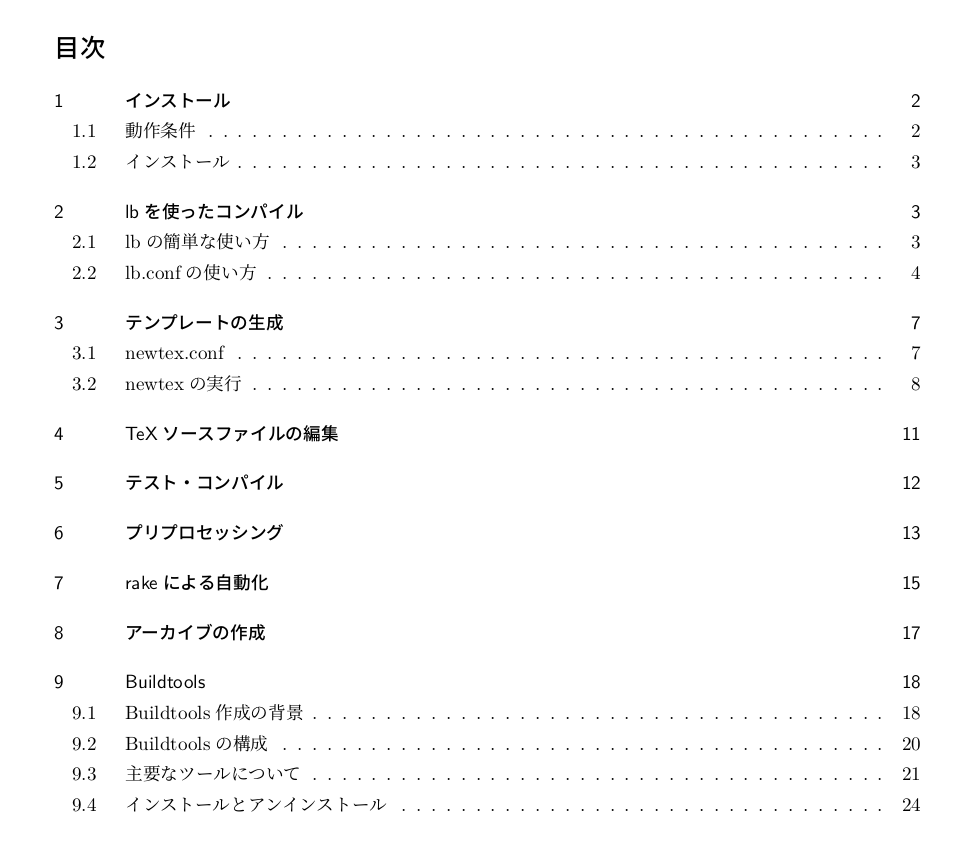
\includegraphics[width=12cm]{tableofcontents.png}
\end{center}

これで、目次にセクション9、そして「Readme.ja.md」の内容が表示された。

このセクションではpandocを手動で走らせた。
もしも、Readme.ja.md がアップグレードされたならば、再びpandocを実行しなければならない。
それは面倒なことであり、本来自動化されるべきことである。
ひとつの方法はRakefileを変更してrakeがコンパイル前に自動的にプリプロセッシングするようにすることである。
次のセクションでその方法を説明する。


\section{rakeによる自動化}
  rakeはmakeに似たビルド・ツールである。
Rakefileには、rakeがソースファイルをビルドする手順が書かれている。
Rakefileには任意のrubyコマンドを記述することができる。
したがって、そのビルドの過程が、たとえ複雑であってもそれを記述することが可能である。

newtexは自動的にRakefileを生成するが、プリプロセッシングが無ければ、そのままで十分使うことができる。
前セクションでは、readme.texを生成するためにpandocを用いたプリプロセッシングが行われた。
したがって、Rakefileを変更してpandocをその中に記述する必要がある。
以下のようにRakefileを変更する。
In the previous section, we used pandoc to generate readme.tex.
So, we need to modify Rakefile to put in pandoc.
Modify the Rakefile as follows.
\begin{verbatim}
require 'rake/clean'

# if readme.tex doesn't exist, generate it first.
# This is necessary because readme.tex is accessed by gfiles in
#  line 12.
if File.exist?("readme.tex") == false
  sh "pandoc -o readme.tex ../Readme.md"
end
# use Latex-BuildTools
@tex_files = (`tfiles -a` + `tfiles -p`).split("\n")
@tex_files <<= "readme.tex"
@graphic_files = []
@tex_files.each do |file|
  @graphic_files += `gfiles #{file}`.split("\n")
end

task default: "チュートリアル.pdf"

file "チュートリアル.pdf" => "_build/main.pdf" do
  sh "cp _build/main.pdf チュートリアル.pdf"
end

file "_build/main.pdf" => (@tex_files+@graphic_files) do
  sh "lb main.tex"
end

file "readme.tex" => "../Readme.ja.md" do
  sh "pandoc -o readme.tex ../Readme.ja.md"
end

CLEAN << "_build"
task :clean

task :ar do
  sh "arl main.tex"
  sh "tar -rf main.tar Rakefile"
  sh "gzip main.tar"
  sh "mv main.tar.gz チュートリアル.tar.gz"
end

task :zip do
  sh "arl -z main.tex"
  sh "zip main.zip Rakefile"
  sh "mv main.zip チュートリアル.zip"
end\end{verbatim}

この変更のおかげで、pandocを手動で走らせる必要はなくなった。
やらなければいけないのは、ただ単に「rake」とタイプするだけである。

rubyとrakeに関するウェブサイトはいくつかある。
例えば、
\begin{itemize}
\item \url{https://www.ruby-lang.org/en/}
\item \url{http://rubylearning.com/}
\item \url{https://ruby.github.io/rake/}
\end{itemize}
がその主なもので、参照してほしい。

\section{アーカイブの作成}
  You might want to distribute your source files.
Then, you need to archive them.
The script `arl' looks for the subfiles and the graphics files included by the rootfile, and archive them.
\begin{itemize}
\item If -g option is given, it makes gzip compressed tarball.
\item If -b option is given, it makes bzip2 compressed tarball.
\item If -z option is given, it makes zip file.
\item If no option is given, it makes non-compressed tarball.
\end{itemize}

If some latex source files are generated by preprocessing, you need to generate them before running arl.
\begin{verbatim}
$ arl
$ tar -tf main.tar
main.tex
edit_tex_files.tex
generate_templates.tex
installation.tex
lb.tex
preprocessing.tex
rake.tex
readme.tex
tarball.tex
test_compile.tex
helper.tex
Tutorial_1.png
Tutorial_2.png
hellolatex.png
tableofcontents.png
test_installation.png
\end{verbatim}

Rakefile needs to be added to the tarball.
\begin{verbatim}
$ tar -rf main.tar Rakefile
\end{verbatim}
Then, compress it into gzip.
\begin{verbatim}
$ gzip main.tar
\end{verbatim}

The procedure above is already written in the Rakefile.
Type `rake ar', then rake makes a tarball.
\begin{verbatim}
$ rm main.tar.gz
$ rake ar
arl main.tex
tar -rf main.tar Rakefile
gzip main.tar
mv main.tar.gz Tutorial.tar.gz
\end{verbatim}
Now the name of the tarball is `Tutorial.tar.gz'.

If you want to make a zip file, type `rake zip'.

The tutorial finishes at this section.
Next section is the copy of Readme.md in Buildtools source files.
It describes the background of Buildtools and features of each script.

\end{document}
\end{verbatim}
最初の行はドキュメントクラスの指定で、newtex.confのdovumentclassキーの値が引数になっている。
2番めの行ではhelper.texを取り込むinputコマンドが書かれている。
helper.texは\verb|\usepackage|コマンドでパッケージを取り込んだり、\verb|\newcommand|コマンドでマクロを定義するなどの役割がある。
プリアンブルの記述のほとんどはhelper.texに書かれている。
ユーザが自分専用のhelper.texを作っておくのは、良い考えである。
というのは、同じプリアンブルをいろいろな文書に使い回すことが多いからである。
自分専用helper.texを持っているユーザはこのテンプレートを上書きすると良い。

4行目は書き直しが必要である。
例えば、
\begin{verbatim}
\author{関谷 敏雄}
\end{verbatim}
のように。
`{\textbackslash}date'、`{\textbackslash}thanks'、abstract環境などを必要に応じて付け加えて良い。
また、目次が必要であれば、8行目のハッシュマークを外して、アンコメントする。
残りの行は、セクションとそのセクションの内容を記述したサブファイルを取り込むための{\textbackslash}inputコマンドである。

Rakefileはrakeに対する指示を書いたファイルである。
当面はこれを書き換える必要はない。
テンプレートをそのまま使い、rakeを実行してみよう。
\begin{verbatim}
$ rake
 ... ...
 ... ...
$ ls
Makefile            generate_templates.tex  preprocessing.tex
Rakefile            helper.tex              rake.tex
_build              installation.tex        tarball.tex
cover.tex           lb.conf                 test_compile.tex
edit_tex_files.tex  lb.tex                  チュートリアル.pdf
gecko.png           main.tex
$ ls _build
main.aux          main.fls  main.out
main.fdb_latexmk  main.log  main.pdf
$ evince Tutorial.pdf
\end{verbatim}
rakeはlbを起動してmain.texをコンパイルし、その後「\_build/main.pdf」を「チュートリアル.pdf」にコピーする。
Evinceは「チュートリアル.pdf」を次のように表示してくれる。
\begin{center}
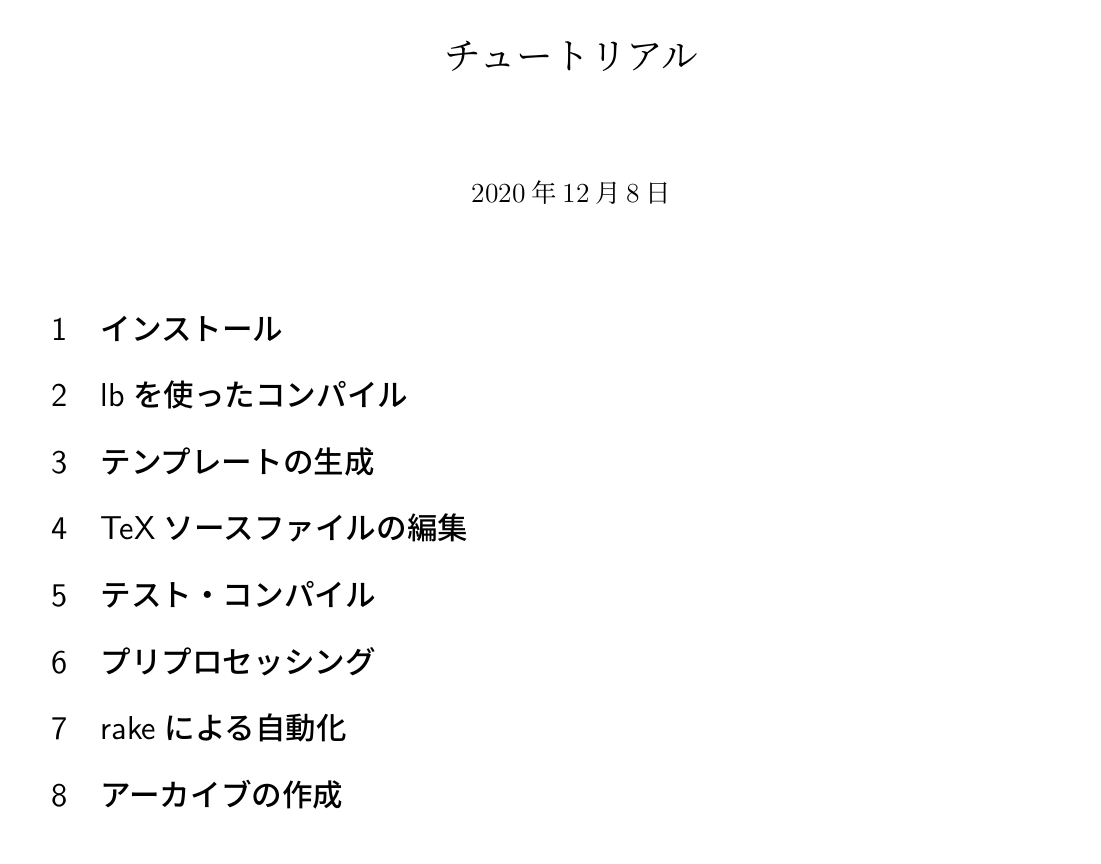
\includegraphics[width=12cm]{Tutorial_1.png}
\end{center}


\section{TeXソースファイルの編集}
  main.texには8つのセクションとそれに対応するサブファイルを取り込む{\textbackslash}inputコマンドが書かれている。
それぞれのサブファイルはテンプレートとして生成された直後は空のファイルである。
そのサブファイルの編集が文書作成の主要な作業になり、作成にかかる時間の大部分がそれに当てられる。

ところで、セクションの編集の途中でも、そこまでをpdfにするとどうなるかを見たいことがあるだろう。
そのためのコンパイルをテスト・コンパイルという。
多くの場合、編集とテスト・コンパイルの間を何回も行ったり来たりしながら、文書作成が進むものである。

もしも、文書がさほど大きくないならば、rakeを用いるのがテスト・コンパイルには最も良い。
というのは、さほどコンパイル時間もかからず、文書全体のpdfを見ることができるからである。
このチュートリアルは、どちらかといえば小さい文書であるから、rakeをテスト・コンパイルに用いるのが良い。

さて、最初のセクションを編集する代わりに、ソースファイル「installation.tex」をコピーしよう。
\begin{verbatim}
\subsection{動作条件}
Buildtoolsには次のものが必要である。
\begin{enumerate}
\item Linux OS とbash
\item LaTeXシステム
\item MakeまたはRake
\end{enumerate}
 ... ...
 ... ...
\end{verbatim}
コピーがすんだら、下記のようにタイプしてpdfを見てみよう。
\begin{verbatim}
$ rake
$ evince チュートリアル.pdf
\end{verbatim}

\begin{center}
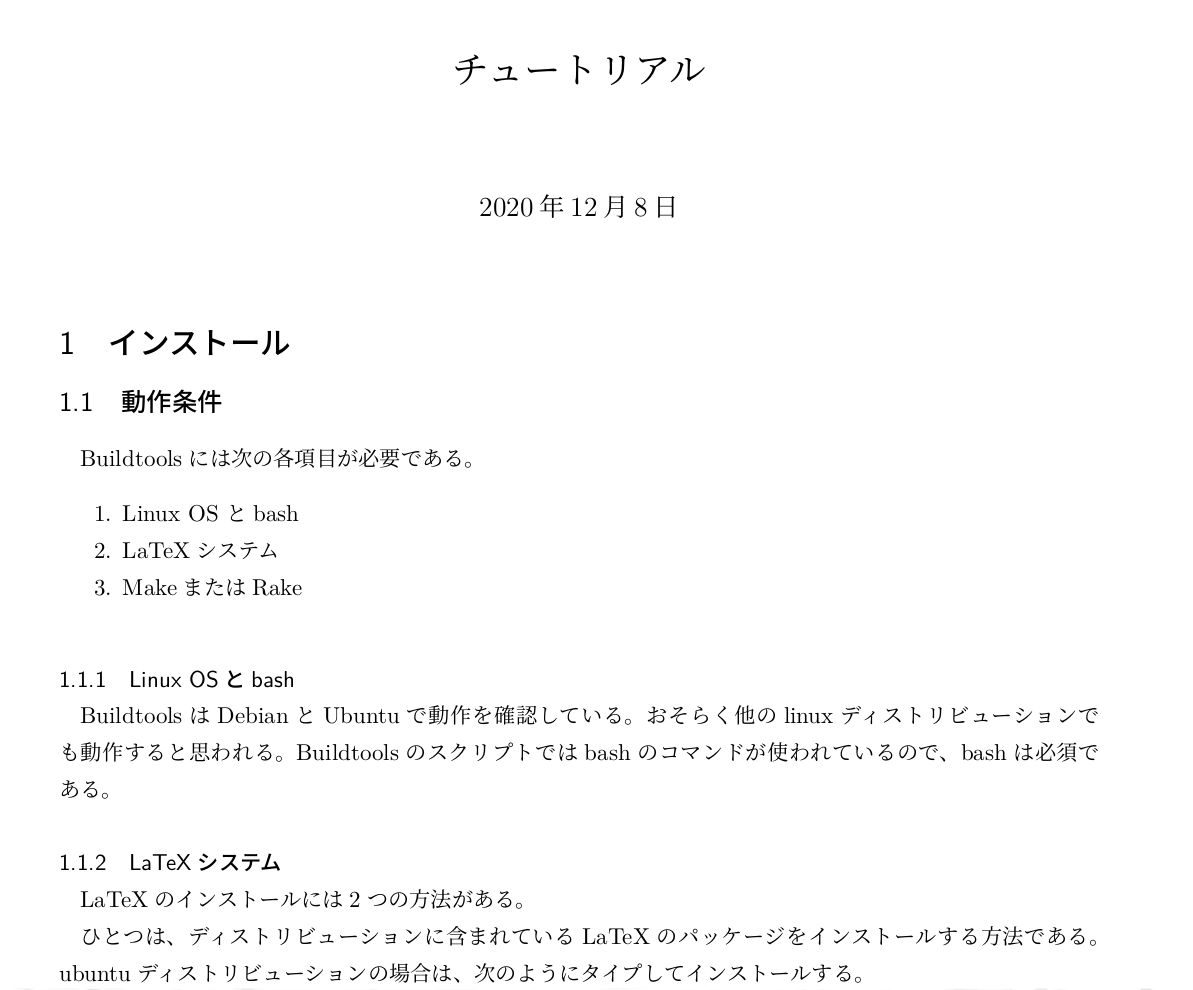
\includegraphics[width=12cm]{Tutorial_2.png}
\end{center}

\section{テスト・コンパイル}
  If you make a big document, for example a book which has more than 100 pages, then using rake is not a good way to test-compile.
The bigger the dicument is, the longer time the compiling takes.

It is a better way to use `lb' to test-compile a subfile separately.
Lb makes a temporary rootfile which includes only the subfile and compile it once.
The advantage of this way is very quick to compile.
However, it has disadvantages.
It only compiles the subfile, so the pdf you get is not a finished document.
It compiles once, so cross-reference doesn't work at all.
It is difficult to say which is better.
it depends on the size of your document.
If it is very big, use lb to test-compile separately.

In this section, I want to show you how to use lb to test-compile a subfile.
This document `Tutorial' is not big, but it's OK.
This is an example to show how to use lb.

Type the following.
\begin{verbatim}
$ lb installation
\end{verbatim}
The argument is a subfile.
The suffix can be left out.
Then, lb makes a temporary rootfile `\_build/test\_installation.tex'.
Its preamble is a copy of the preamble in the original rootfile.
It has {\textbackslash}input command and includes the subfile `installation.tex'.
Lb compiles `\_build/test\_installation.tex' and run the previewer specified in `lb.conf' to show the pdf.
\begin{center}
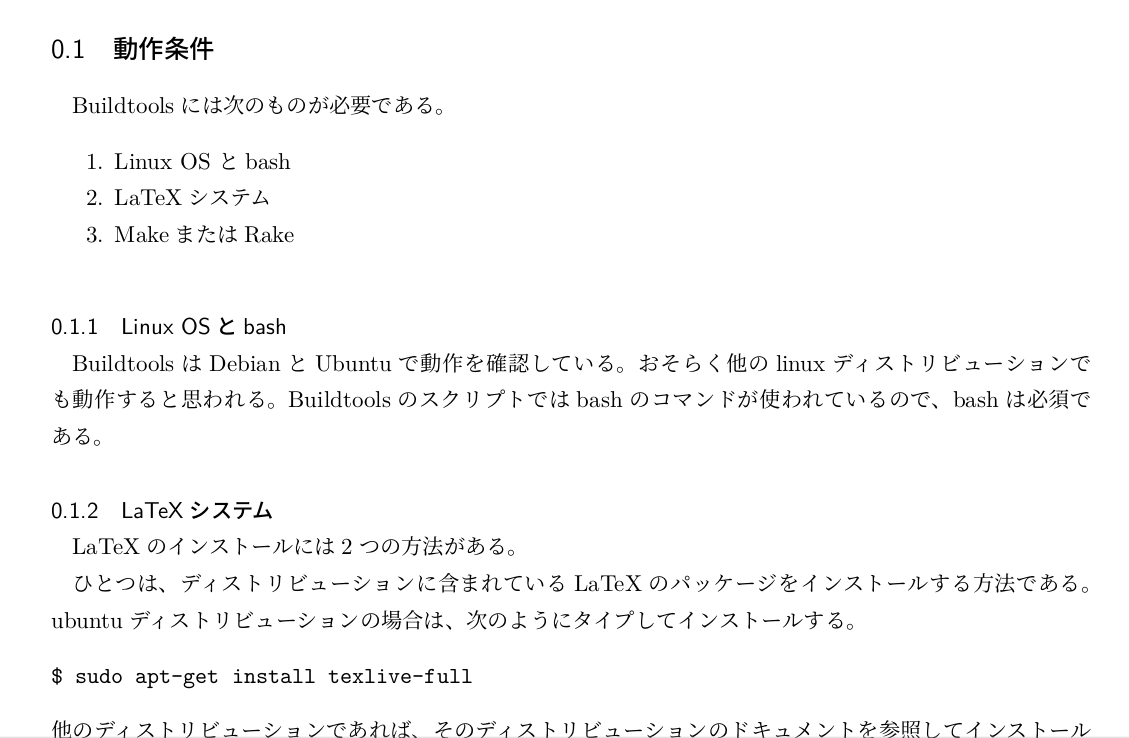
\includegraphics[width=12cm]{test_installation.png}
\end{center}

Lb compiles a subfile with the option synctex on.
Therefore, if you open the source files, `\_build/test\_installation.tex' and `installation.tex' in this example, you can do forward search and backward search between the source and pdf.
If your use gedit and evince, backward search works by clicking left button with pressing down CTRL key, but forward search from `installation.tex' doesn't work.
If you want to do it, add the following line at the beginning of the subfile.
\begin{verbatim}
% mainfile: _build/test_installation.tex
\end{verbatim}
However, forward search isn't used so often compared to backward search.
Adding the line above is usually unnecessary.


\section{プリプロセッシング}
  ときにはlatexソースファイルをコンパイルする前に何かしておきたい、ということがあるかもしれない。
例えば、
\begin{itemize}
\item gnuplotなどのプログラムを使って画像ファイルを生成したい
\item pandocを使ってlatexソースファイルを自動生成したい
\end{itemize}

このチュートリアルではプリプロセッサとしてpandocを使う方法を紹介したい。
pandocは文書コンバータである。
markdown、latex、html、pdfなど多くの種類の文書を変換することができる。
このチュートリアルでは、Buildtoolsのソースファイルの中にある「Readme.ja.md」を「readme.tex」というlatexソースファイルに変換してみる。

たいていのディストリビューションではpandocパッケージが備わっているので、インストールは簡単である。
例えばubuntuでは
\begin{verbatim}
$ sudo apt-get install pandoc
\end{verbatim}
でインストールできる。

readme.texを生成するには次のようにタイプする。
\begin{verbatim}
$ pandoc -o readme.tex ../Readme.ja.md
\end{verbatim}

この他に2つほどmain.texとhelper.texに変更を加える必要がある。
まず、{\textbackslash}inputコマンドを用いてreadme.texを取り込む命令をmain.texの最後に記述する。
\begin{verbatim}
\documentclass{article}
% helper.tex

% You need to rewrite this file to fit your build environment.

% Notice
% The driver of graphicx package is luatex.
% If you use another engine, then you need to rewrite it to your driver.
% For example, if you use pdflatex, then the driver is pdftex.

% Packages
\usepackage{amsmath,amssymb}
\usepackage[luatex]{graphicx}
\usepackage{tikz}
\usetikzlibrary{calc}
\usetikzlibrary{topaths}
\usetikzlibrary{plotmarks}
\usetikzlibrary{intersections}
\usetikzlibrary{arrows,decorations.pathmorphing,backgrounds,positioning,fit,petri}
\usetikzlibrary{arrows.meta}
\usetikzlibrary{3d}

\usepackage{fancybox}
\usepackage{booktabs}

\usepackage[margin=2.4cm]{geometry}

\usepackage[colorlinks=true,linkcolor=black]{hyperref}

% Sample macro.
%\newcommand{\solution}{\begin{flushleft}\textbf{Solution:}\end{flushleft}}
%\newcommand{\proof}{\begin{flushleft}\textbf{Proof}\end{flushleft}}
%\newcommand{\qed}{\begin{flushright}\textbf{q. e. d.}\end{flushright}}
%\newcommand{\answer}[1]{\begin{flushleft}\textbf{Exercise~\ref{#1}}\end{flushleft}}

% Theorem environment.
%\newtheorem{theorem}{Theorem}[section]
%\newtheorem{lemma}{Lemma}[section]
%\newtheorem{corollary}{Corollary}[section]
%\newtheorem{definition}{Definition}[section]
%\newtheorem{example}{Example}[section]
%\newtheorem{exercise}{Exercise}[section]

 ... ...
 ... ...
\section{Make tarball}
  You might want to distribute your source files.
Then, you need to archive them.
The script `arl' looks for the subfiles and the graphics files included by the rootfile, and archive them.
\begin{itemize}
\item If -g option is given, it makes gzip compressed tarball.
\item If -b option is given, it makes bzip2 compressed tarball.
\item If -z option is given, it makes zip file.
\item If no option is given, it makes non-compressed tarball.
\end{itemize}

If some latex source files are generated by preprocessing, you need to generate them before running arl.
\begin{verbatim}
$ arl
$ tar -tf main.tar
main.tex
edit_tex_files.tex
generate_templates.tex
installation.tex
lb.tex
preprocessing.tex
rake.tex
readme.tex
tarball.tex
test_compile.tex
helper.tex
Tutorial_1.png
Tutorial_2.png
hellolatex.png
tableofcontents.png
test_installation.png
\end{verbatim}

Rakefile needs to be added to the tarball.
\begin{verbatim}
$ tar -rf main.tar Rakefile
\end{verbatim}
Then, compress it into gzip.
\begin{verbatim}
$ gzip main.tar
\end{verbatim}

The procedure above is already written in the Rakefile.
Type `rake ar', then rake makes a tarball.
\begin{verbatim}
$ rm main.tar.gz
$ rake ar
arl main.tex
tar -rf main.tar Rakefile
gzip main.tar
mv main.tar.gz Tutorial.tar.gz
\end{verbatim}
Now the name of the tarball is `Tutorial.tar.gz'.

If you want to make a zip file, type `rake zip'.

The tutorial finishes at this section.
Next section is the copy of Readme.md in Buildtools source files.
It describes the background of Buildtools and features of each script.

\hypertarget{buildtools}{%
\section{Buildtools}\label{buildtools}}

\hypertarget{the-background-of-buildtools}{%
\subsection{The background of
Buildtools}\label{the-background-of-buildtools}}

\hypertarget{buildtools-is-a-part-of-latextools}{%
\paragraph{Buildtools is a part of
Latextools}\label{buildtools-is-a-part-of-latextools}}

If you make a long document, for example, a book with more than a
hundred pages, you need to consider various things which isn't necessary
in creating a short document.

\begin{itemize}
\tightlist
\item
  Divide the source file into small parts
\item
  Compile each parts independently
\item
  Replace something with another in the whole document
\item
  Preprocessing (processes before compiling latex source files)
\end{itemize}

Latextools support these things and it includes two parts.

\begin{itemize}
\tightlist
\item
  Buildtools. It is tools which support creating templates of source
  files, building and partial compiling.
\item
  Substools. It is tools which perform replacements in the whole
  document.
\end{itemize}

Buildtools is a part of Latextools and also a core tools in it. This
document describes Buildtools only.

\hypertarget{dividing-a-source-file}{%
\paragraph{Dividing a source file}\label{dividing-a-source-file}}

Latex source files are simply called source files here. It is not
appropriate to write a long document into a single source file. Because,
bigger the file, much more difficult to edit it. To solve this, the
document will be divided into some parts. Usually, they consist of a
file containing \texttt{\textbackslash{}begin\{document\}} and
\texttt{\textbackslash{}end\{document\}} and the other files called by
the file with \texttt{\textbackslash{}include} or
\texttt{\textbackslash{}input} command. The former file is called
rootfile and the latter files are called subfiles. There is a difference
between \texttt{\textbackslash{}include} and
\texttt{\textbackslash{}input} though both are commands to include
subfiles.

\begin{itemize}
\item
  \texttt{\textbackslash{}include} can't be nested. it can be described
  only in the body, which means the part between
  \texttt{\textbackslash{}begin\{document\}} and
  \texttt{\textbackslash{}end\{document\}}.
  \texttt{\textbackslash{}includeonly}, which must be in the preamble,
  specifies a list of files to include by the
  \texttt{\textbackslash{}include} command. The files in the list are
  included by \texttt{\textbackslash{}include} command, and files out of
  the list aren't included even if it is an argument of
  \texttt{\textbackslash{}include} command.
  \texttt{\textbackslash{}include} command issues
  \texttt{\textbackslash{}clearpage} command before and after including
  the file.
\item
  \texttt{\textbackslash{}input} command simply include files. It
  doesn't issue \texttt{\textbackslash{}clearpage} command. This command
  can be nested.
\end{itemize}

It is called build to make a document by compiling. It includes not only
the compilation with latex but also the preprocessing, such as the image
generation by gnuplot or tikz graph generation with data. It is finally
completed by the compilation of the rootfile.

There are several programs to compile LaTeX source files, and they are
called engines. Buildtools supports latex, platex, pdflatex, xelatex and
lualate as engines.

The bigger the document to compile is, the longer the time needs. Even
if you change a small part of the document, it needs the same time as
the big change. You often need to compile to check how the pdf document
looks like, which is sometimes called test, it needs long time in each
compilation. The bigger the document is, the more serious the problem
is. So, it has been thought up to compile a subfile itself without
rootfile or other subfiles.

\begin{itemize}
\tightlist
\item
  Comment out the files in the argument list of
  \texttt{\textbackslash{}includeonly} command which you don't want to
  compile.
\item
  Use subfiles package.
\end{itemize}

Subfiles package is nice and many people recommend it. However, you need
to include the package and use its command appropriately. Naturally, it
is not the matter compared with the compilation time above.

Another way is to add an specific preamble to compile a subfile without
any other files. More specifically, the subfile is put between ``the
text from \texttt{\textbackslash{}documentclass} to
\texttt{\textbackslash{}begin\{document\}}'' and
``\texttt{\textbackslash{}end\{document\}}''. On that occasion, the
subfile itself isn't changed, but another file, which contains the
preamble, \texttt{\textbackslash{}end\{document\}} and
\texttt{\textbackslash{}input} command, is made. The
\texttt{\textbackslash{}input} command reads the subfile. The file newly
made is called ``temporary rootfile''. On the other hand, the rootfile
is sometimes called " original rootfile". The preamble in the temporary
rootfile is a copy of the preamble in the original rootfile. The good
point of this way is:

\begin{itemize}
\tightlist
\item
  There's no need to include any packages or put any special commands.
\item
  Therefore, users don't need to install any packages when the source
  file is distributed.
\end{itemize}

The point is subfile can be compiled separately without any modification
in the source files. The generation of the temporary rootfile is the
only necessary. Buildtools has \texttt{ttex} shell script to do that.

\hypertarget{repeating-compiling}{%
\paragraph{Repeating compiling}\label{repeating-compiling}}

It often needs to compile source files two times or more because of the
cross-reference. The repeating times are maybe two or three (or more),
but I don't know the details. However, there's a great software that
calculate the repeating times automatically. It is latexmk. Latexmk make
the build very easy. Buildtools uses latexmk to compile rootfiles.

\hypertarget{build-directory}{%
\paragraph{Build directory}\label{build-directory}}

Some people might complain about latex because it generates various of
auxiliary files and log files. If you make a build directory and put all
the generated files into it, the source directory can be kept clean. One
of such program is cluttex and it is recommended to people who like
cleanliness.

Buildtools makes a temporary directory, which is also called build
directory, and put all the temporary files and generated document. The
default name of the directory is \texttt{\_build}. It makes the source
directory keep clean. If you want to see log or auxiliary files, search
the build directory for them. It's very simple. Although it is
superfluous to say so, meson build system which is very popular as a C
build tool also uses build directory. This shows us that separating
build directory from source directory is very easy to understand.

Lb, one of the tools in Buildtools, generate a final pdf document in the
build directory. However, many users probably want to put it in the
source directory. It is a natural idea. If you want to do so, use make
or rake.

Rake is a similar program to make. Its advantage is using ruby language
in the Rakefile, which is the script file of rake. Because ruby language
is very strong and flexible, the script file can be readable and
structured.

To get back to the subject how to put a final pdf document in the source
directory, you just write a cp command in your Makefile or Rakefile to
copy the pdf document under the build directory into source directory.
Furthermore, the advantage to use make or rake is that it's possible to
specify preprocessing code in the Makefile or Rakefile. Because
preprocessing depends on the document and what tools the user choose,
it's difficult for Buildtools to cover the preprocessing. Compared with
that, Makefile or Rakefile are really flexible so that you can write
your own preprocessing in it.

It is recommended that users should use make or rake with Buildtools.

\hypertarget{combination-with-texworks}{%
\paragraph{combination with Texworks}\label{combination-with-texworks}}

Lb, one of the tools in Buildtools, can either compile a rootfile or
test-compile a subfile. If you specify it into proccessing tools in the
texworks dialog, you can run lb from texworks and it's so convenient.
Click edit, preference, then typesetting tab. Click plus button in the
processing tools part, then put \texttt{lb}, \texttt{lb},
\texttt{\$fullname} in name, program and arguments box respectively.
Once you set it, you can compile a rootfile or test-compile a subfile by
clicking on the typesetting icon (green triangle icon).

\hypertarget{buildtools-structure}{%
\subsection{Buildtools structure}\label{buildtools-structure}}

Buildtools is made up of the following five parts.

\begin{itemize}
\tightlist
\item
  \texttt{newtex}: It generates source file templates. This is used at
  the beginning of making documents.
\item
  \texttt{lb}: It calls latexmk or ttex to compile source files.
\item
  \texttt{arl}: It makes an archive file.
\item
  installer
\item
  a group of utilities. They are used by the tools above.
\end{itemize}

The following shows the steps to build documents.

\begin{enumerate}
\def\labelenumi{\arabic{enumi}.}
\tightlist
\item
  Make the structure, especially the chapters/sections, of the
  document..
\item
  Run newtex and make folders and templates of the document.
\item
  Modify the templates of Makefile, Rakefile, cover page (cover.tex) and
  preamble (cover.tex) if necessary.
\item
  Write the body of the document and test-compile.
\item
  If necessary, make script files for the preprocessing.
\item
  Compile the rootfile to generate the final pdf document.
\end{enumerate}

The step three to five above are usually repeated and the process is not
necessarily in the order above.

\hypertarget{main-tools}{%
\subsection{Main tools}\label{main-tools}}

Each tool shows its help message if it is run with \texttt{-\/-help}
option. For example, newtex shows the following message.

\begin{verbatim}
$ newtex --help
Usage:
  newtex --help
    Show this message.
  Newtex.conf needs to be edited before running newtex.
  newtex
    A directory is made and some template files are generated under the directory.
\end{verbatim}

The document of each tool is:

\begin{itemize}
\tightlist
\item
  The help message shown by each command with \texttt{-\/-help} option.
\item
  The description below in this document.
\end{itemize}

No other document exists. If you want to know more, see the source code.
All the tools in Buildtools are shell scripts. If you are familiar to
shell scripts, you can easily understand them because they are short.

\hypertarget{newtex}{%
\paragraph{newtex}\label{newtex}}

\begin{verbatim}
$ newtex
\end{verbatim}

Newtex is used when you make a new latex document. irst, decide the
structure and chapters and make \texttt{newtex.conf} in advance. This
script makes a directory and generates template files according to
\texttt{newtex.conf}.

\begin{enumerate}
\def\labelenumi{\arabic{enumi}.}
\tightlist
\item
  There is \texttt{newtex.conf} file in the Buildtools source files.
  Modify it to fit your environment and tex source files you will make.
\item
  Execute \texttt{newtex}. Then it make a directory which name is the
  same as \texttt{title} in \texttt{newtex.conf}. However, the space
  characters in the value of \texttt{title} is converted to underscore
  in the name of the directory. The script also generates template files
  under the directory.
\end{enumerate}

\hypertarget{lb}{%
\paragraph{lb}\label{lb}}

\begin{verbatim}
$ lb [LaTeXfile]
\end{verbatim}

If the argument is left out, \texttt{lb} behaves as if \texttt{main.tex}
is specified as an argument. \texttt{Lb} is a script to build LaTeX
source files and you usually don't need anything except it.

\begin{itemize}
\tightlist
\item
  If the argument is rootfile, then \texttt{lb} compiles it with
  \texttt{latexmk}. If the argument is subfile, then \texttt{lb} runs
  \texttt{ttex} specifying the subfile as an argument.
\item
  If the argument is rootfile, \texttt{lb} compiles it without synctex.
\item
  If the argument is subfile, \texttt{lb} runs \texttt{ttex} and
  \texttt{ttex} compiles the subfile with synctex. After compilation,
  \texttt{lb} runs previewer specified in \texttt{lb.conf}.
\item
  If there exists \texttt{lb.conf} in the current directory (it usually
  contains the rootfile), \texttt{lb} reads it and initialize some
  variables.
\item
  If the variable \texttt{engine} in \texttt{lb.conf} is null string,
  then \texttt{lb} guesses an appropriate engine by itself. However, it
  is recommended that you should specify the engine in \texttt{lb.conf}.
\end{itemize}

You can specify the default values in \texttt{lb.conf} to initialize
some variables.

\begin{verbatim}
rootfile=main.tex
builddir=_build
engine=
latex_option=-halt-on-error
preview=texworks
\end{verbatim}

\begin{itemize}
\tightlist
\item
  \texttt{rootfile} is the name of the rootfile. If you specify the name
  of the rootfile as an argument to \texttt{lb}, then the argument takes
  precedence.
\item
  \texttt{builddir} is the name of the build directory. Auxiliary files
  and output files are put in the build directory. If the argument of
  \texttt{lb} is a subfile, then the temporary rootfile is also put in
  the build directory. If \texttt{builddir} is empty, then no temporary
  directory is generated and the source file directory becomes a build
  directory.
\item
  \texttt{engine} is the name of a latex engine. \texttt{latex},
  \texttt{platex}, \texttt{pdflatex}, \texttt{xelatex} and
  \texttt{lualatex} can be specified. Other engines are not supported.
\item
  \texttt{latex\_option} is a list of options to specify as an argument
  to the engine through \texttt{latexmk}. \texttt{-output-directory} is
  automatically given to \texttt{latexmk} by \texttt{lb} even if
  \texttt{lb.conf}doesn't exist.
\item
  \texttt{preview} is the name of a pdf previewer to show the document.
  It is run only if the argument of \texttt{lb} is a subfile.
\end{itemize}

\hypertarget{arl}{%
\paragraph{arl}\label{arl}}

\$ arl {[}-b\textbar{}-g\textbar{}-z{]} {[}rootfile{]}

The name \texttt{arl} comes from ``ARchive LaTeX files''. It searches
the rootfile for its related files (refer the following) and make an
archive file. If the argument is left out, then it runs as if
\texttt{main.tex} is specified as an argument.

\begin{itemize}
\tightlist
\item
  If there are preprocessing programs, you need to execute them before
  running arl.
\item
  Arl archives the latex source files and the graphic files included by
  \texttt{\textbackslash{}includegraphics} command.
\item
  Therefore, \texttt{Makefile} or the preprocessing script files are not
  archived.
\end{itemize}

It is a good way to make a target (for example, its name is `ar') in
Makefile and write a recipe to add Makefile and the preprocessing files
into the archive file made by \texttt{arl}. You can do the same thing
with Rakefile.

There are options \texttt{-g}, \texttt{-b} and \texttt{-z} to compress
the archive file into \texttt{tar.gz}, \texttt{tar.bz2} and \texttt{zip}
file respectively. If no option is given, \texttt{arl} just make a
tarball without compression.

\hypertarget{utilities}{%
\paragraph{Utilities}\label{utilities}}

You don't need to read this subsection except maintaining the scripts.

\begin{verbatim}
$ srf subfile
\end{verbatim}

This script \texttt{srf} searches for the rootfile of the given subfile
and outputs its absolute path. \texttt{srf} comes from ``Search for Root
File''.

\begin{verbatim}
$ tfiles [-p|-a|-i] [rootfile]
\end{verbatim}

It outputs a list of subfiles of the given rootfile. If the argument is
left out, then it is run as if \texttt{main.tex} is specified as an
argument.

\begin{itemize}
\tightlist
\item
  No option: It outputs a list of subfiles, specified from
  \texttt{\textbackslash{}begin\{document\}} to
  \texttt{\textbackslash{}end\{document\}}. They are the arguments of
  \texttt{\textbackslash{}include} or \texttt{\textbackslash{}input}
  command.
\item
  \texttt{-p}: It outputs a list of subfiles specified with the
  \texttt{\textbackslash{}input} commands in the preamble of the
  rootfile.
\item
  \texttt{-a}: It outputs a list, outputted with no option, and the
  rootfile itself.
\item
  \texttt{-i}: It outputs a list of subfiles specified with both
  \texttt{\textbackslash{}include} and
  \texttt{\textbackslash{}includeonly} command.
\end{itemize}

The files in the list are separated with new lines.

\begin{verbatim}
$ tftype [-r|-s|-q] files ...
\end{verbatim}

It outputs or returns the type of the given latex files.

\begin{itemize}
\tightlist
\item
  \texttt{-r}: It outputs rootfiles which is in the argument files. If
  no options are given, It behaves as if this option is specified.
\item
  \texttt{-s}: It outputs subfiles which is in the argument files.
\item
  \texttt{-q}: It doesn't output anything. The number of the argument
  must be one. It returns an exit status code of the file type. If the
  code is 0 or 1, then the file is a rootfile or subfile respectively.
  Otherwise an error happens.
\end{itemize}

Using \texttt{-q} option is the most common.

\begin{verbatim}
$ gfiles files ...
\end{verbatim}

The argument is a list of latex source files. It outputs graphic files
which are included by \texttt{\textbackslash{}includegraphics} commands
in the given files.

\begin{verbatim}
$ ltxengine rootfile
\end{verbatim}

It guesses a latex engine to compile the rootfile, although it is
recommended that the engine should be specified by the user. For
example,

\begin{verbatim}
\usepackage[luatex]{graphicx}
\end{verbatim}

If this command exists in the preamble, it guesses that the engine is
probably lualatex.

\begin{verbatim}
$ ttex [-b builddir] -e latex_engine [-p dvipdf] [-v previewr] -r rootfile subfile
\end{verbatim}

It generates a temporary rootfile of the subfile and compile it. The
compilation is done only once. Therefore, no cross-reference is carried
out. This comes from the idea that \texttt{ttex} is a script for test to
see how the pdf file looks like and cross-reference is not so important.
The cross-reference to the other files doesn't work neither. This script
can be run directly on the command line, but usually it is called by
\texttt{lb}. The following shows the options.

\begin{itemize}
\tightlist
\item
  \texttt{-b}: Specify a build directory. The default is
  \texttt{\_build}.
\item
  \texttt{-e}: Specify a latex engine. There is no restriction on the
  engine, but it assumes that latex, platex, pdflatex, xelatex or
  lualatex is specified.
\item
  \texttt{-p}: Specify an application that translates dvi into pdf. This
  is used only when the engine is latex or platex, because they outputs
  a dvi file. The default is dvipdfmx. Other possible application is
  dvipdfm and dvipdf.
\item
  \texttt{-v}: Specify a pdf previewer like evince. If you edit the
  source file with texworks, it is a good idea to specify texworks here.
\item
  \texttt{-r}: Specify the original rootfile.
\end{itemize}

\hypertarget{installation-and-uninstallation}{%
\subsection{Installation and
uninstallation}\label{installation-and-uninstallation}}

\hypertarget{prerequisite}{%
\paragraph{Prerequisite}\label{prerequisite}}

\begin{itemize}
\item
  Linux and bash: It is tested on Debian and Ubuntu. However, it
  probably works on other linux distributions. Bash is required because
  this script includes bash commands.
\item
  LaTeX: There are two options to install LaTeX. One is installing the
  LaTeX applications provided by your distribution. The other is
  installing TexLive.
\item
  make or rake: These applications are not necessarily required to run
  the tools in Buildtools. However, it is recommended that they are used
  under the control of make or rake. You don't need to install both of
  them. Choose one which you like. Make is a traditional build tool
  originally aimed at C compiler. Rake is a build tool similar to make.
  It is one of the ruby application. The advantage to use rake is that
  you can put any ruby codes into Rakefile, which is the script file of
  rake. Generally speaking, Rakefile is easy to understand than
  Makefile.
\end{itemize}

\hypertarget{installation}{%
\paragraph{Installation}\label{installation}}

Use the script install.sh.

\begin{verbatim}
$ bash install.sh
\end{verbatim}

This script installs the executable files into \texttt{\$HOME/bin}.
Debian and Ubuntu adds the directory \texttt{\$HOME/bin} into
\texttt{PATH} environment variable if it exists at the login time. The
script makes the directory \texttt{\$HOME/bin} if it doesn't exist. In
that case, you need to re-login to put the directory into the
\texttt{PATH} environment variable. If you run \texttt{sudo} or
\texttt{su} to become the root user before the installation, the
executable files are put into \texttt{/user/local/bin}.

If your OS is debian, type the following to be the root user.

\begin{verbatim}
$ su -
# bash install.sh
\end{verbatim}

Or if it's ubuntu,

\begin{verbatim}
$ sudo bash install.sh
\end{verbatim}

\hypertarget{uninstallation}{%
\paragraph{Uninstallation}\label{uninstallation}}

Use the script uninstall.sh.

\begin{verbatim}
$ bash uninstall.sh
\end{verbatim}

If you run this as a user, the files under \texttt{\$HOME} are removed.
If you run this as a root, the files under \texttt{/usr/local} are
removed. If your OS is debian, type the following to be the root user.

\begin{verbatim}
$ su -
# bash uninstall.sh
\end{verbatim}

Or if it's ubuntu,

\begin{verbatim}
$ sudo bash uninstall.sh
\end{verbatim}

\hypertarget{licence}{%
\subsection{licence}\label{licence}}

Copyright (C) 2020 ToshioCP (Toshio Sekiya)

Buildtools is free software; you can redistribute it and/or modify it
under the terms of the GNU General Public License as published by the
Free Software Foundation; either version 3 of the License, or (at your
option) any later version.

Buildtools is distributed in the hope that it will be useful, but
WITHOUT ANY WARRANTY; without even the implied warranty of
MERCHANTABILITY or FITNESS FOR A PARTICULAR PURPOSE. See the
\href{https://www.gnu.org/licenses/gpl-3.0.html}{GNU Lesser General
Public License} for more details.

\end{document}
\end{verbatim}
更に、8行目の{\textbackslash}tableofcontentsをアンコメントしてコマンドが利くようにしよう。
\begin{verbatim}
 ... ...
\maketitle
% If you want a table of contents here, uncomment the following
 line.
\tableofcontents
 ... ...
\end{verbatim}

2番めは、{\textbackslash}tightlistのマクロを定義することが必要である。
Helper.texがその定義を書くのに最も適した場所である。
\begin{verbatim}
 ... ...
 ... ...
\providecommand{\tightlist}{%
  \setlength{\itemsep}{0pt}\setlength{\parskip}{0pt}}
 ... ...
 ... ...
\end{verbatim}
このコードは\url{https://github.com/jgm/pandoc-templates/blob/master/default.latex}から引用したものである。

rakeを使ってコンパイルする。
\begin{verbatim}
$ rake
\end{verbatim}

\begin{center}
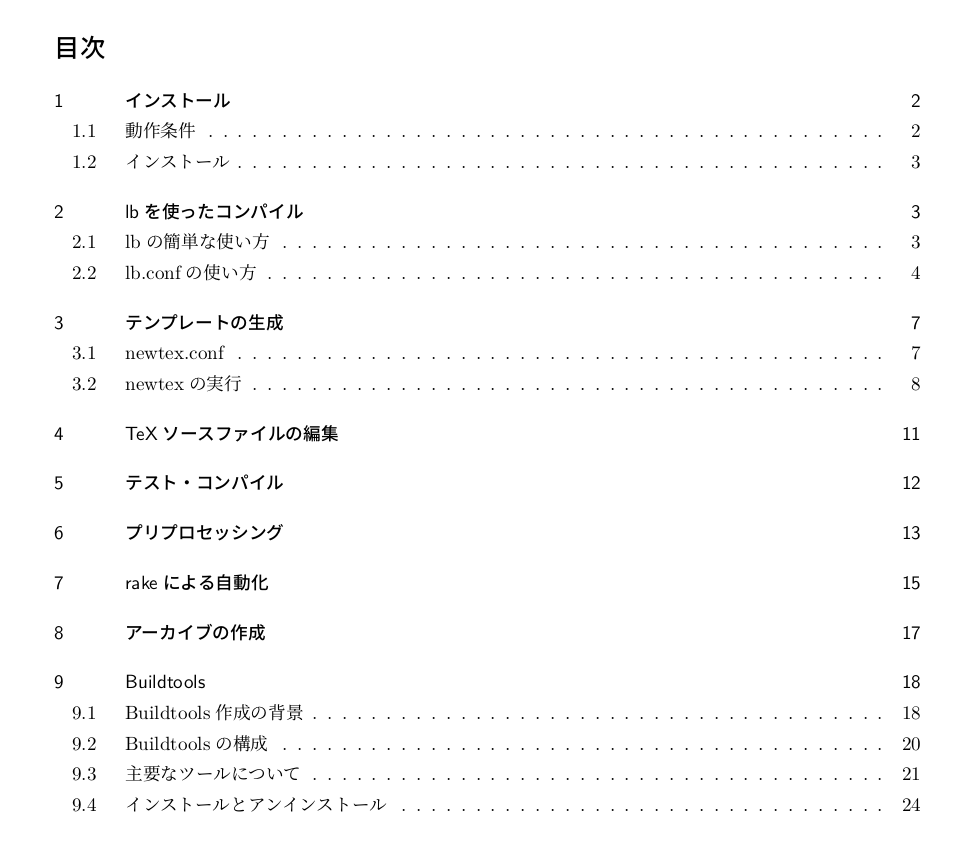
\includegraphics[width=12cm]{tableofcontents.png}
\end{center}

これで、目次にセクション9、そして「Readme.ja.md」の内容が表示された。

このセクションではpandocを手動で走らせた。
もしも、Readme.ja.md がアップグレードされたならば、再びpandocを実行しなければならない。
それは面倒なことであり、本来自動化されるべきことである。
ひとつの方法はRakefileを変更してrakeがコンパイル前に自動的にプリプロセッシングするようにすることである。
次のセクションでその方法を説明する。


\section{rakeによる自動化}
  rakeはmakeに似たビルド・ツールである。
Rakefileには、rakeがソースファイルをビルドする手順が書かれている。
Rakefileには任意のrubyコマンドを記述することができる。
したがって、そのビルドの過程が、たとえ複雑であってもそれを記述することが可能である。

newtexは自動的にRakefileを生成するが、プリプロセッシングが無ければ、そのままで十分使うことができる。
前セクションでは、readme.texを生成するためにpandocを用いたプリプロセッシングが行われた。
したがって、Rakefileを変更してpandocをその中に記述する必要がある。
以下のようにRakefileを変更する。
In the previous section, we used pandoc to generate readme.tex.
So, we need to modify Rakefile to put in pandoc.
Modify the Rakefile as follows.
\begin{verbatim}
require 'rake/clean'

# if readme.tex doesn't exist, generate it first.
# This is necessary because readme.tex is accessed by gfiles in
#  line 12.
if File.exist?("readme.tex") == false
  sh "pandoc -o readme.tex ../Readme.md"
end
# use Latex-BuildTools
@tex_files = (`tfiles -a` + `tfiles -p`).split("\n")
@tex_files <<= "readme.tex"
@graphic_files = []
@tex_files.each do |file|
  @graphic_files += `gfiles #{file}`.split("\n")
end

task default: "チュートリアル.pdf"

file "チュートリアル.pdf" => "_build/main.pdf" do
  sh "cp _build/main.pdf チュートリアル.pdf"
end

file "_build/main.pdf" => (@tex_files+@graphic_files) do
  sh "lb main.tex"
end

file "readme.tex" => "../Readme.ja.md" do
  sh "pandoc -o readme.tex ../Readme.ja.md"
end

CLEAN << "_build"
task :clean

task :ar do
  sh "arl main.tex"
  sh "tar -rf main.tar Rakefile"
  sh "gzip main.tar"
  sh "mv main.tar.gz チュートリアル.tar.gz"
end

task :zip do
  sh "arl -z main.tex"
  sh "zip main.zip Rakefile"
  sh "mv main.zip チュートリアル.zip"
end\end{verbatim}

この変更のおかげで、pandocを手動で走らせる必要はなくなった。
やらなければいけないのは、ただ単に「rake」とタイプするだけである。

rubyとrakeに関するウェブサイトはいくつかある。
例えば、
\begin{itemize}
\item \url{https://www.ruby-lang.org/en/}
\item \url{http://rubylearning.com/}
\item \url{https://ruby.github.io/rake/}
\end{itemize}
がその主なもので、参照してほしい。

\section{アーカイブの作成}
  You might want to distribute your source files.
Then, you need to archive them.
The script `arl' looks for the subfiles and the graphics files included by the rootfile, and archive them.
\begin{itemize}
\item If -g option is given, it makes gzip compressed tarball.
\item If -b option is given, it makes bzip2 compressed tarball.
\item If -z option is given, it makes zip file.
\item If no option is given, it makes non-compressed tarball.
\end{itemize}

If some latex source files are generated by preprocessing, you need to generate them before running arl.
\begin{verbatim}
$ arl
$ tar -tf main.tar
main.tex
edit_tex_files.tex
generate_templates.tex
installation.tex
lb.tex
preprocessing.tex
rake.tex
readme.tex
tarball.tex
test_compile.tex
helper.tex
Tutorial_1.png
Tutorial_2.png
hellolatex.png
tableofcontents.png
test_installation.png
\end{verbatim}

Rakefile needs to be added to the tarball.
\begin{verbatim}
$ tar -rf main.tar Rakefile
\end{verbatim}
Then, compress it into gzip.
\begin{verbatim}
$ gzip main.tar
\end{verbatim}

The procedure above is already written in the Rakefile.
Type `rake ar', then rake makes a tarball.
\begin{verbatim}
$ rm main.tar.gz
$ rake ar
arl main.tex
tar -rf main.tar Rakefile
gzip main.tar
mv main.tar.gz Tutorial.tar.gz
\end{verbatim}
Now the name of the tarball is `Tutorial.tar.gz'.

If you want to make a zip file, type `rake zip'.

The tutorial finishes at this section.
Next section is the copy of Readme.md in Buildtools source files.
It describes the background of Buildtools and features of each script.

\hypertarget{buildtools}{%
\section{Buildtools}\label{buildtools}}

\hypertarget{the-background-of-buildtools}{%
\subsection{The background of
Buildtools}\label{the-background-of-buildtools}}

\hypertarget{buildtools-is-a-part-of-latextools}{%
\paragraph{Buildtools is a part of
Latextools}\label{buildtools-is-a-part-of-latextools}}

If you make a long document, for example, a book with more than a
hundred pages, you need to consider various things which isn't necessary
in creating a short document.

\begin{itemize}
\tightlist
\item
  Divide the source file into small parts
\item
  Compile each parts independently
\item
  Replace something with another in the whole document
\item
  Preprocessing (processes before compiling latex source files)
\end{itemize}

Latextools support these things and it includes two parts.

\begin{itemize}
\tightlist
\item
  Buildtools. It is tools which support creating templates of source
  files, building and partial compiling.
\item
  Substools. It is tools which perform replacements in the whole
  document.
\end{itemize}

Buildtools is a part of Latextools and also a core tools in it. This
document describes Buildtools only.

\hypertarget{dividing-a-source-file}{%
\paragraph{Dividing a source file}\label{dividing-a-source-file}}

Latex source files are simply called source files here. It is not
appropriate to write a long document into a single source file. Because,
bigger the file, much more difficult to edit it. To solve this, the
document will be divided into some parts. Usually, they consist of a
file containing \texttt{\textbackslash{}begin\{document\}} and
\texttt{\textbackslash{}end\{document\}} and the other files called by
the file with \texttt{\textbackslash{}include} or
\texttt{\textbackslash{}input} command. The former file is called
rootfile and the latter files are called subfiles. There is a difference
between \texttt{\textbackslash{}include} and
\texttt{\textbackslash{}input} though both are commands to include
subfiles.

\begin{itemize}
\item
  \texttt{\textbackslash{}include} can't be nested. it can be described
  only in the body, which means the part between
  \texttt{\textbackslash{}begin\{document\}} and
  \texttt{\textbackslash{}end\{document\}}.
  \texttt{\textbackslash{}includeonly}, which must be in the preamble,
  specifies a list of files to include by the
  \texttt{\textbackslash{}include} command. The files in the list are
  included by \texttt{\textbackslash{}include} command, and files out of
  the list aren't included even if it is an argument of
  \texttt{\textbackslash{}include} command.
  \texttt{\textbackslash{}include} command issues
  \texttt{\textbackslash{}clearpage} command before and after including
  the file.
\item
  \texttt{\textbackslash{}input} command simply include files. It
  doesn't issue \texttt{\textbackslash{}clearpage} command. This command
  can be nested.
\end{itemize}

It is called build to make a document by compiling. It includes not only
the compilation with latex but also the preprocessing, such as the image
generation by gnuplot or tikz graph generation with data. It is finally
completed by the compilation of the rootfile.

There are several programs to compile LaTeX source files, and they are
called engines. Buildtools supports latex, platex, pdflatex, xelatex and
lualate as engines.

The bigger the document to compile is, the longer the time needs. Even
if you change a small part of the document, it needs the same time as
the big change. You often need to compile to check how the pdf document
looks like, which is sometimes called test, it needs long time in each
compilation. The bigger the document is, the more serious the problem
is. So, it has been thought up to compile a subfile itself without
rootfile or other subfiles.

\begin{itemize}
\tightlist
\item
  Comment out the files in the argument list of
  \texttt{\textbackslash{}includeonly} command which you don't want to
  compile.
\item
  Use subfiles package.
\end{itemize}

Subfiles package is nice and many people recommend it. However, you need
to include the package and use its command appropriately. Naturally, it
is not the matter compared with the compilation time above.

Another way is to add an specific preamble to compile a subfile without
any other files. More specifically, the subfile is put between ``the
text from \texttt{\textbackslash{}documentclass} to
\texttt{\textbackslash{}begin\{document\}}'' and
``\texttt{\textbackslash{}end\{document\}}''. On that occasion, the
subfile itself isn't changed, but another file, which contains the
preamble, \texttt{\textbackslash{}end\{document\}} and
\texttt{\textbackslash{}input} command, is made. The
\texttt{\textbackslash{}input} command reads the subfile. The file newly
made is called ``temporary rootfile''. On the other hand, the rootfile
is sometimes called " original rootfile". The preamble in the temporary
rootfile is a copy of the preamble in the original rootfile. The good
point of this way is:

\begin{itemize}
\tightlist
\item
  There's no need to include any packages or put any special commands.
\item
  Therefore, users don't need to install any packages when the source
  file is distributed.
\end{itemize}

The point is subfile can be compiled separately without any modification
in the source files. The generation of the temporary rootfile is the
only necessary. Buildtools has \texttt{ttex} shell script to do that.

\hypertarget{repeating-compiling}{%
\paragraph{Repeating compiling}\label{repeating-compiling}}

It often needs to compile source files two times or more because of the
cross-reference. The repeating times are maybe two or three (or more),
but I don't know the details. However, there's a great software that
calculate the repeating times automatically. It is latexmk. Latexmk make
the build very easy. Buildtools uses latexmk to compile rootfiles.

\hypertarget{build-directory}{%
\paragraph{Build directory}\label{build-directory}}

Some people might complain about latex because it generates various of
auxiliary files and log files. If you make a build directory and put all
the generated files into it, the source directory can be kept clean. One
of such program is cluttex and it is recommended to people who like
cleanliness.

Buildtools makes a temporary directory, which is also called build
directory, and put all the temporary files and generated document. The
default name of the directory is \texttt{\_build}. It makes the source
directory keep clean. If you want to see log or auxiliary files, search
the build directory for them. It's very simple. Although it is
superfluous to say so, meson build system which is very popular as a C
build tool also uses build directory. This shows us that separating
build directory from source directory is very easy to understand.

Lb, one of the tools in Buildtools, generate a final pdf document in the
build directory. However, many users probably want to put it in the
source directory. It is a natural idea. If you want to do so, use make
or rake.

Rake is a similar program to make. Its advantage is using ruby language
in the Rakefile, which is the script file of rake. Because ruby language
is very strong and flexible, the script file can be readable and
structured.

To get back to the subject how to put a final pdf document in the source
directory, you just write a cp command in your Makefile or Rakefile to
copy the pdf document under the build directory into source directory.
Furthermore, the advantage to use make or rake is that it's possible to
specify preprocessing code in the Makefile or Rakefile. Because
preprocessing depends on the document and what tools the user choose,
it's difficult for Buildtools to cover the preprocessing. Compared with
that, Makefile or Rakefile are really flexible so that you can write
your own preprocessing in it.

It is recommended that users should use make or rake with Buildtools.

\hypertarget{combination-with-texworks}{%
\paragraph{combination with Texworks}\label{combination-with-texworks}}

Lb, one of the tools in Buildtools, can either compile a rootfile or
test-compile a subfile. If you specify it into proccessing tools in the
texworks dialog, you can run lb from texworks and it's so convenient.
Click edit, preference, then typesetting tab. Click plus button in the
processing tools part, then put \texttt{lb}, \texttt{lb},
\texttt{\$fullname} in name, program and arguments box respectively.
Once you set it, you can compile a rootfile or test-compile a subfile by
clicking on the typesetting icon (green triangle icon).

\hypertarget{buildtools-structure}{%
\subsection{Buildtools structure}\label{buildtools-structure}}

Buildtools is made up of the following five parts.

\begin{itemize}
\tightlist
\item
  \texttt{newtex}: It generates source file templates. This is used at
  the beginning of making documents.
\item
  \texttt{lb}: It calls latexmk or ttex to compile source files.
\item
  \texttt{arl}: It makes an archive file.
\item
  installer
\item
  a group of utilities. They are used by the tools above.
\end{itemize}

The following shows the steps to build documents.

\begin{enumerate}
\def\labelenumi{\arabic{enumi}.}
\tightlist
\item
  Make the structure, especially the chapters/sections, of the
  document..
\item
  Run newtex and make folders and templates of the document.
\item
  Modify the templates of Makefile, Rakefile, cover page (cover.tex) and
  preamble (cover.tex) if necessary.
\item
  Write the body of the document and test-compile.
\item
  If necessary, make script files for the preprocessing.
\item
  Compile the rootfile to generate the final pdf document.
\end{enumerate}

The step three to five above are usually repeated and the process is not
necessarily in the order above.

\hypertarget{main-tools}{%
\subsection{Main tools}\label{main-tools}}

Each tool shows its help message if it is run with \texttt{-\/-help}
option. For example, newtex shows the following message.

\begin{verbatim}
$ newtex --help
Usage:
  newtex --help
    Show this message.
  Newtex.conf needs to be edited before running newtex.
  newtex
    A directory is made and some template files are generated under the directory.
\end{verbatim}

The document of each tool is:

\begin{itemize}
\tightlist
\item
  The help message shown by each command with \texttt{-\/-help} option.
\item
  The description below in this document.
\end{itemize}

No other document exists. If you want to know more, see the source code.
All the tools in Buildtools are shell scripts. If you are familiar to
shell scripts, you can easily understand them because they are short.

\hypertarget{newtex}{%
\paragraph{newtex}\label{newtex}}

\begin{verbatim}
$ newtex
\end{verbatim}

Newtex is used when you make a new latex document. irst, decide the
structure and chapters and make \texttt{newtex.conf} in advance. This
script makes a directory and generates template files according to
\texttt{newtex.conf}.

\begin{enumerate}
\def\labelenumi{\arabic{enumi}.}
\tightlist
\item
  There is \texttt{newtex.conf} file in the Buildtools source files.
  Modify it to fit your environment and tex source files you will make.
\item
  Execute \texttt{newtex}. Then it make a directory which name is the
  same as \texttt{title} in \texttt{newtex.conf}. However, the space
  characters in the value of \texttt{title} is converted to underscore
  in the name of the directory. The script also generates template files
  under the directory.
\end{enumerate}

\hypertarget{lb}{%
\paragraph{lb}\label{lb}}

\begin{verbatim}
$ lb [LaTeXfile]
\end{verbatim}

If the argument is left out, \texttt{lb} behaves as if \texttt{main.tex}
is specified as an argument. \texttt{Lb} is a script to build LaTeX
source files and you usually don't need anything except it.

\begin{itemize}
\tightlist
\item
  If the argument is rootfile, then \texttt{lb} compiles it with
  \texttt{latexmk}. If the argument is subfile, then \texttt{lb} runs
  \texttt{ttex} specifying the subfile as an argument.
\item
  If the argument is rootfile, \texttt{lb} compiles it without synctex.
\item
  If the argument is subfile, \texttt{lb} runs \texttt{ttex} and
  \texttt{ttex} compiles the subfile with synctex. After compilation,
  \texttt{lb} runs previewer specified in \texttt{lb.conf}.
\item
  If there exists \texttt{lb.conf} in the current directory (it usually
  contains the rootfile), \texttt{lb} reads it and initialize some
  variables.
\item
  If the variable \texttt{engine} in \texttt{lb.conf} is null string,
  then \texttt{lb} guesses an appropriate engine by itself. However, it
  is recommended that you should specify the engine in \texttt{lb.conf}.
\end{itemize}

You can specify the default values in \texttt{lb.conf} to initialize
some variables.

\begin{verbatim}
rootfile=main.tex
builddir=_build
engine=
latex_option=-halt-on-error
preview=texworks
\end{verbatim}

\begin{itemize}
\tightlist
\item
  \texttt{rootfile} is the name of the rootfile. If you specify the name
  of the rootfile as an argument to \texttt{lb}, then the argument takes
  precedence.
\item
  \texttt{builddir} is the name of the build directory. Auxiliary files
  and output files are put in the build directory. If the argument of
  \texttt{lb} is a subfile, then the temporary rootfile is also put in
  the build directory. If \texttt{builddir} is empty, then no temporary
  directory is generated and the source file directory becomes a build
  directory.
\item
  \texttt{engine} is the name of a latex engine. \texttt{latex},
  \texttt{platex}, \texttt{pdflatex}, \texttt{xelatex} and
  \texttt{lualatex} can be specified. Other engines are not supported.
\item
  \texttt{latex\_option} is a list of options to specify as an argument
  to the engine through \texttt{latexmk}. \texttt{-output-directory} is
  automatically given to \texttt{latexmk} by \texttt{lb} even if
  \texttt{lb.conf}doesn't exist.
\item
  \texttt{preview} is the name of a pdf previewer to show the document.
  It is run only if the argument of \texttt{lb} is a subfile.
\end{itemize}

\hypertarget{arl}{%
\paragraph{arl}\label{arl}}

\$ arl {[}-b\textbar{}-g\textbar{}-z{]} {[}rootfile{]}

The name \texttt{arl} comes from ``ARchive LaTeX files''. It searches
the rootfile for its related files (refer the following) and make an
archive file. If the argument is left out, then it runs as if
\texttt{main.tex} is specified as an argument.

\begin{itemize}
\tightlist
\item
  If there are preprocessing programs, you need to execute them before
  running arl.
\item
  Arl archives the latex source files and the graphic files included by
  \texttt{\textbackslash{}includegraphics} command.
\item
  Therefore, \texttt{Makefile} or the preprocessing script files are not
  archived.
\end{itemize}

It is a good way to make a target (for example, its name is `ar') in
Makefile and write a recipe to add Makefile and the preprocessing files
into the archive file made by \texttt{arl}. You can do the same thing
with Rakefile.

There are options \texttt{-g}, \texttt{-b} and \texttt{-z} to compress
the archive file into \texttt{tar.gz}, \texttt{tar.bz2} and \texttt{zip}
file respectively. If no option is given, \texttt{arl} just make a
tarball without compression.

\hypertarget{utilities}{%
\paragraph{Utilities}\label{utilities}}

You don't need to read this subsection except maintaining the scripts.

\begin{verbatim}
$ srf subfile
\end{verbatim}

This script \texttt{srf} searches for the rootfile of the given subfile
and outputs its absolute path. \texttt{srf} comes from ``Search for Root
File''.

\begin{verbatim}
$ tfiles [-p|-a|-i] [rootfile]
\end{verbatim}

It outputs a list of subfiles of the given rootfile. If the argument is
left out, then it is run as if \texttt{main.tex} is specified as an
argument.

\begin{itemize}
\tightlist
\item
  No option: It outputs a list of subfiles, specified from
  \texttt{\textbackslash{}begin\{document\}} to
  \texttt{\textbackslash{}end\{document\}}. They are the arguments of
  \texttt{\textbackslash{}include} or \texttt{\textbackslash{}input}
  command.
\item
  \texttt{-p}: It outputs a list of subfiles specified with the
  \texttt{\textbackslash{}input} commands in the preamble of the
  rootfile.
\item
  \texttt{-a}: It outputs a list, outputted with no option, and the
  rootfile itself.
\item
  \texttt{-i}: It outputs a list of subfiles specified with both
  \texttt{\textbackslash{}include} and
  \texttt{\textbackslash{}includeonly} command.
\end{itemize}

The files in the list are separated with new lines.

\begin{verbatim}
$ tftype [-r|-s|-q] files ...
\end{verbatim}

It outputs or returns the type of the given latex files.

\begin{itemize}
\tightlist
\item
  \texttt{-r}: It outputs rootfiles which is in the argument files. If
  no options are given, It behaves as if this option is specified.
\item
  \texttt{-s}: It outputs subfiles which is in the argument files.
\item
  \texttt{-q}: It doesn't output anything. The number of the argument
  must be one. It returns an exit status code of the file type. If the
  code is 0 or 1, then the file is a rootfile or subfile respectively.
  Otherwise an error happens.
\end{itemize}

Using \texttt{-q} option is the most common.

\begin{verbatim}
$ gfiles files ...
\end{verbatim}

The argument is a list of latex source files. It outputs graphic files
which are included by \texttt{\textbackslash{}includegraphics} commands
in the given files.

\begin{verbatim}
$ ltxengine rootfile
\end{verbatim}

It guesses a latex engine to compile the rootfile, although it is
recommended that the engine should be specified by the user. For
example,

\begin{verbatim}
\usepackage[luatex]{graphicx}
\end{verbatim}

If this command exists in the preamble, it guesses that the engine is
probably lualatex.

\begin{verbatim}
$ ttex [-b builddir] -e latex_engine [-p dvipdf] [-v previewr] -r rootfile subfile
\end{verbatim}

It generates a temporary rootfile of the subfile and compile it. The
compilation is done only once. Therefore, no cross-reference is carried
out. This comes from the idea that \texttt{ttex} is a script for test to
see how the pdf file looks like and cross-reference is not so important.
The cross-reference to the other files doesn't work neither. This script
can be run directly on the command line, but usually it is called by
\texttt{lb}. The following shows the options.

\begin{itemize}
\tightlist
\item
  \texttt{-b}: Specify a build directory. The default is
  \texttt{\_build}.
\item
  \texttt{-e}: Specify a latex engine. There is no restriction on the
  engine, but it assumes that latex, platex, pdflatex, xelatex or
  lualatex is specified.
\item
  \texttt{-p}: Specify an application that translates dvi into pdf. This
  is used only when the engine is latex or platex, because they outputs
  a dvi file. The default is dvipdfmx. Other possible application is
  dvipdfm and dvipdf.
\item
  \texttt{-v}: Specify a pdf previewer like evince. If you edit the
  source file with texworks, it is a good idea to specify texworks here.
\item
  \texttt{-r}: Specify the original rootfile.
\end{itemize}

\hypertarget{installation-and-uninstallation}{%
\subsection{Installation and
uninstallation}\label{installation-and-uninstallation}}

\hypertarget{prerequisite}{%
\paragraph{Prerequisite}\label{prerequisite}}

\begin{itemize}
\item
  Linux and bash: It is tested on Debian and Ubuntu. However, it
  probably works on other linux distributions. Bash is required because
  this script includes bash commands.
\item
  LaTeX: There are two options to install LaTeX. One is installing the
  LaTeX applications provided by your distribution. The other is
  installing TexLive.
\item
  make or rake: These applications are not necessarily required to run
  the tools in Buildtools. However, it is recommended that they are used
  under the control of make or rake. You don't need to install both of
  them. Choose one which you like. Make is a traditional build tool
  originally aimed at C compiler. Rake is a build tool similar to make.
  It is one of the ruby application. The advantage to use rake is that
  you can put any ruby codes into Rakefile, which is the script file of
  rake. Generally speaking, Rakefile is easy to understand than
  Makefile.
\end{itemize}

\hypertarget{installation}{%
\paragraph{Installation}\label{installation}}

Use the script install.sh.

\begin{verbatim}
$ bash install.sh
\end{verbatim}

This script installs the executable files into \texttt{\$HOME/bin}.
Debian and Ubuntu adds the directory \texttt{\$HOME/bin} into
\texttt{PATH} environment variable if it exists at the login time. The
script makes the directory \texttt{\$HOME/bin} if it doesn't exist. In
that case, you need to re-login to put the directory into the
\texttt{PATH} environment variable. If you run \texttt{sudo} or
\texttt{su} to become the root user before the installation, the
executable files are put into \texttt{/user/local/bin}.

If your OS is debian, type the following to be the root user.

\begin{verbatim}
$ su -
# bash install.sh
\end{verbatim}

Or if it's ubuntu,

\begin{verbatim}
$ sudo bash install.sh
\end{verbatim}

\hypertarget{uninstallation}{%
\paragraph{Uninstallation}\label{uninstallation}}

Use the script uninstall.sh.

\begin{verbatim}
$ bash uninstall.sh
\end{verbatim}

If you run this as a user, the files under \texttt{\$HOME} are removed.
If you run this as a root, the files under \texttt{/usr/local} are
removed. If your OS is debian, type the following to be the root user.

\begin{verbatim}
$ su -
# bash uninstall.sh
\end{verbatim}

Or if it's ubuntu,

\begin{verbatim}
$ sudo bash uninstall.sh
\end{verbatim}

\hypertarget{licence}{%
\subsection{licence}\label{licence}}

Copyright (C) 2020 ToshioCP (Toshio Sekiya)

Buildtools is free software; you can redistribute it and/or modify it
under the terms of the GNU General Public License as published by the
Free Software Foundation; either version 3 of the License, or (at your
option) any later version.

Buildtools is distributed in the hope that it will be useful, but
WITHOUT ANY WARRANTY; without even the implied warranty of
MERCHANTABILITY or FITNESS FOR A PARTICULAR PURPOSE. See the
\href{https://www.gnu.org/licenses/gpl-3.0.html}{GNU Lesser General
Public License} for more details.

\end{document}
